%!TEX root = ../diffusion_paper.tex
\section{Results} % (fold)
\label{sec:results}
  \subsection{TDS on Synthetic Geometries} % (fold)
  \label{sub:tds_on_synthetic_geometries}
  \begin{figure}[!t]
    \centering
    \subfloat[]{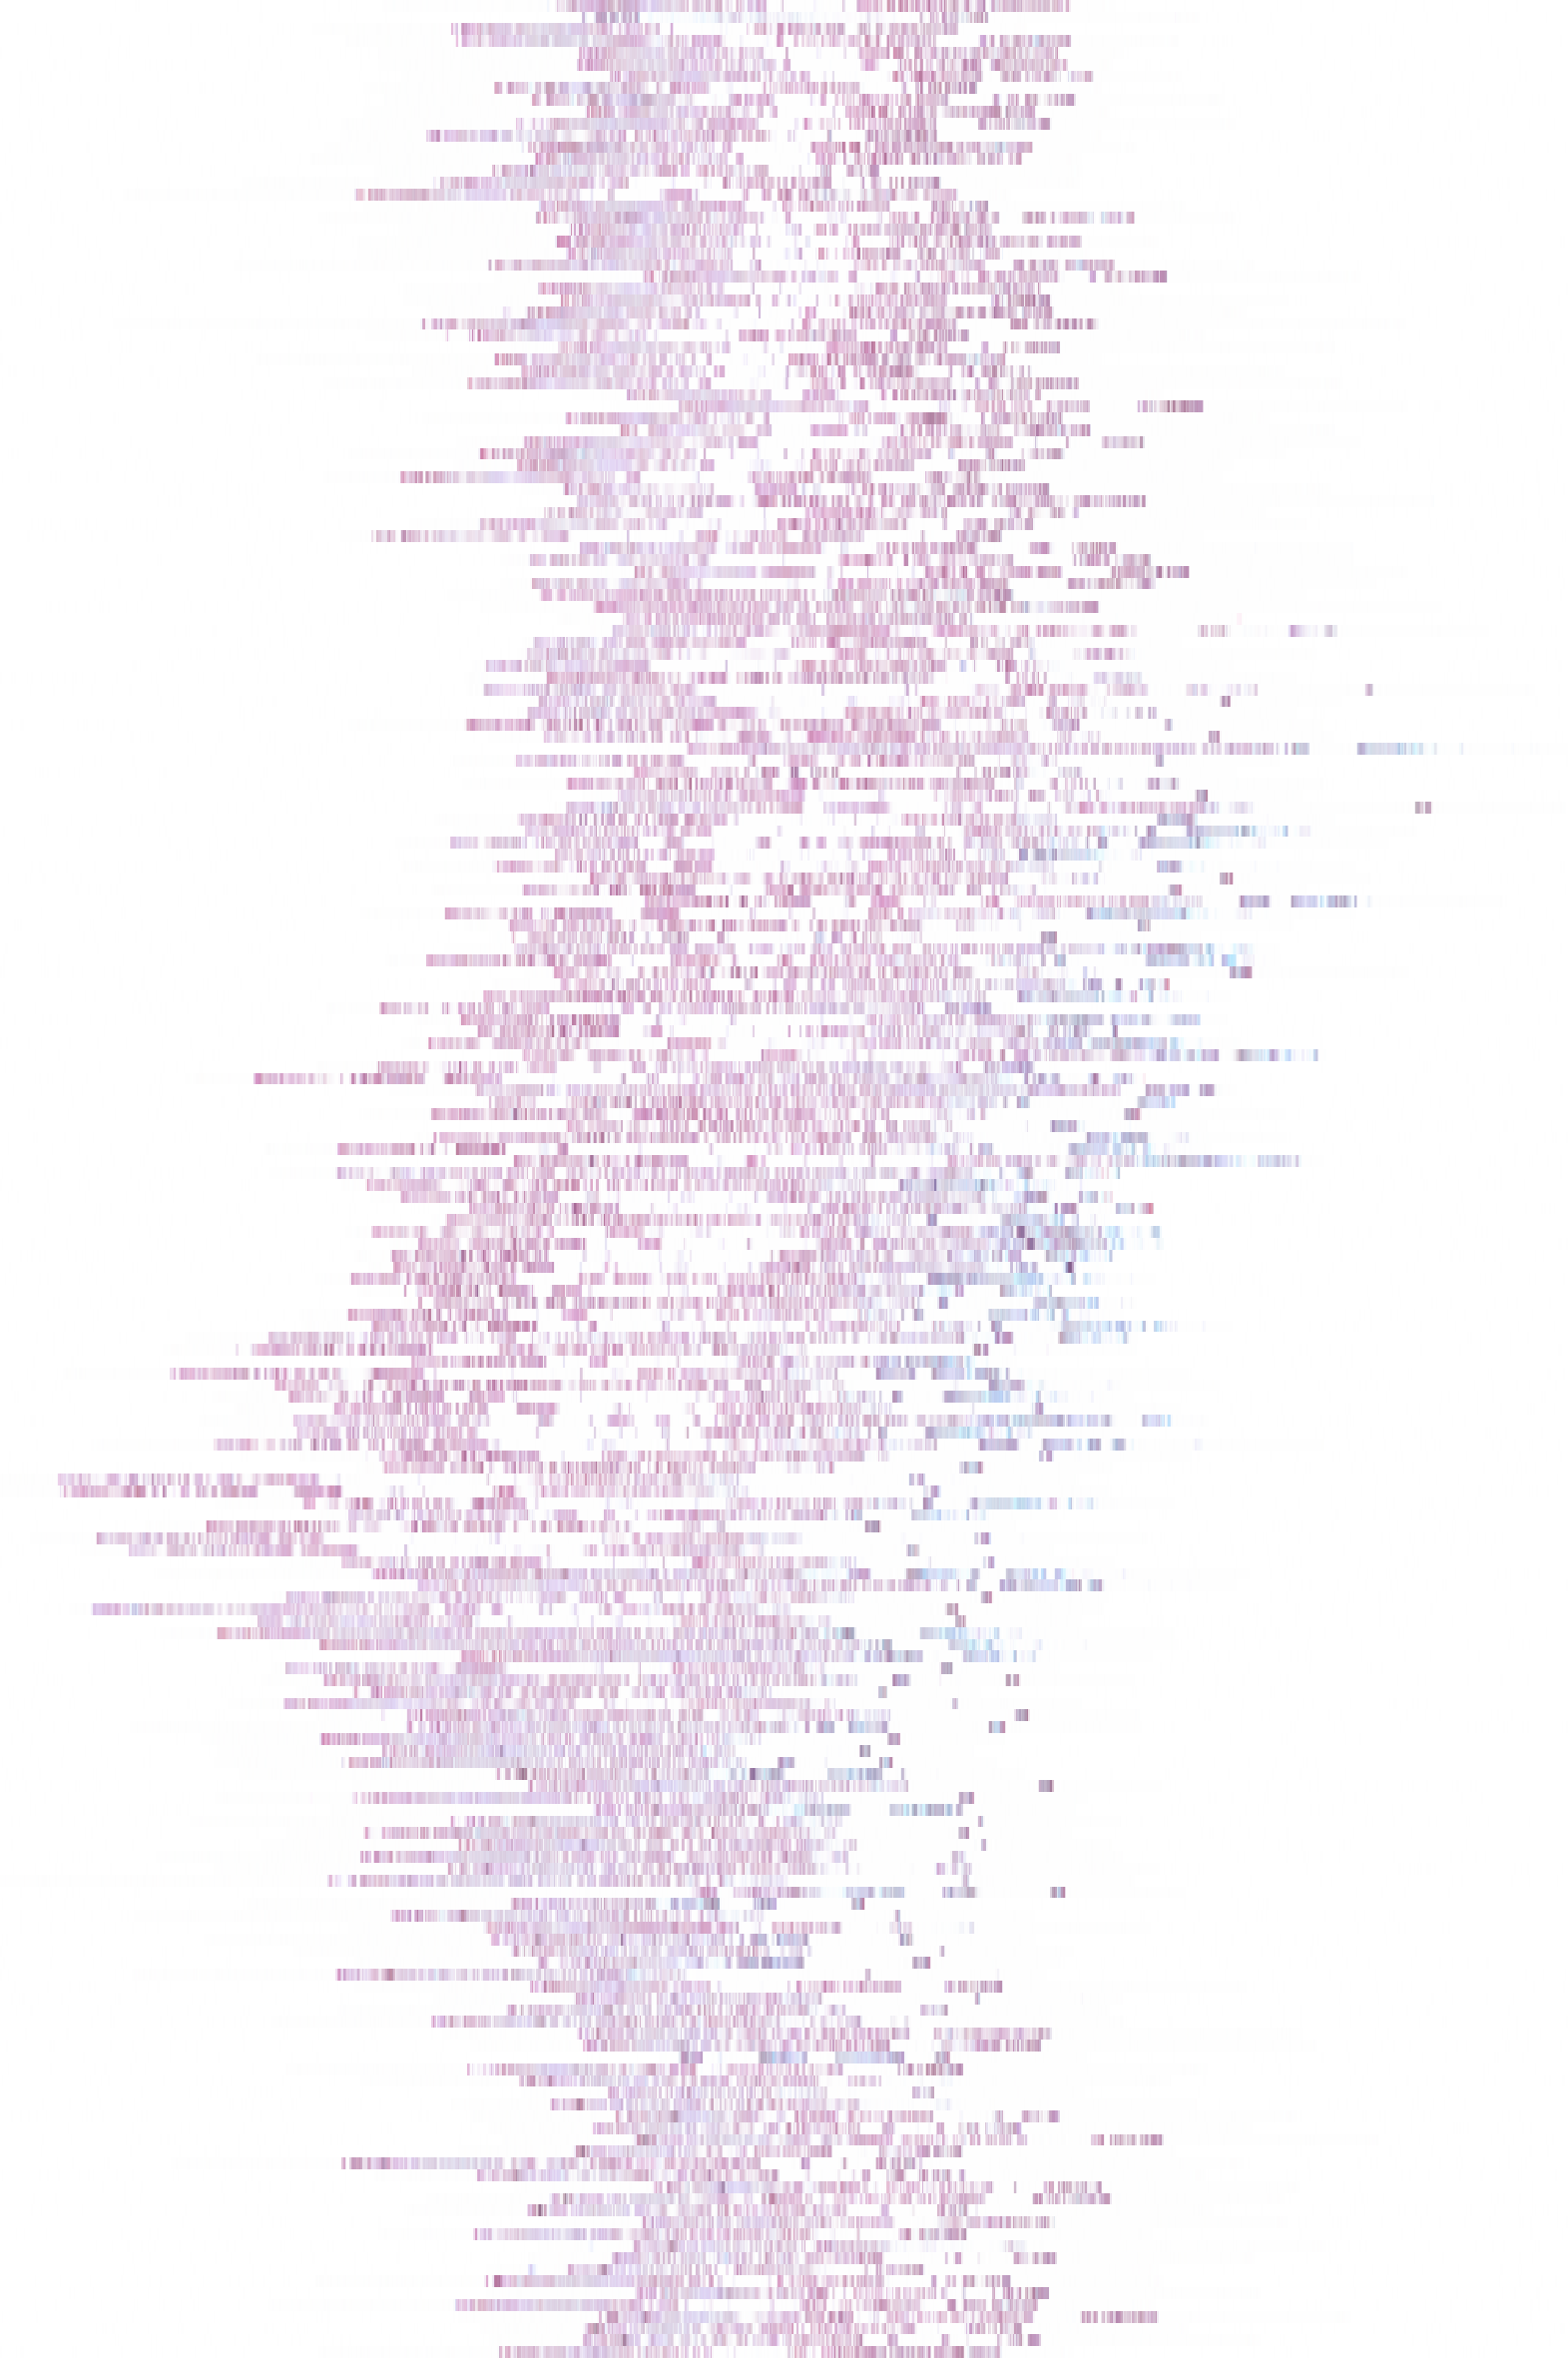
\includegraphics[width=1.1in]{2_methods/Figs/cross_section_0}\label{fig:synthetic_cross_section_0}}
    \subfloat[]{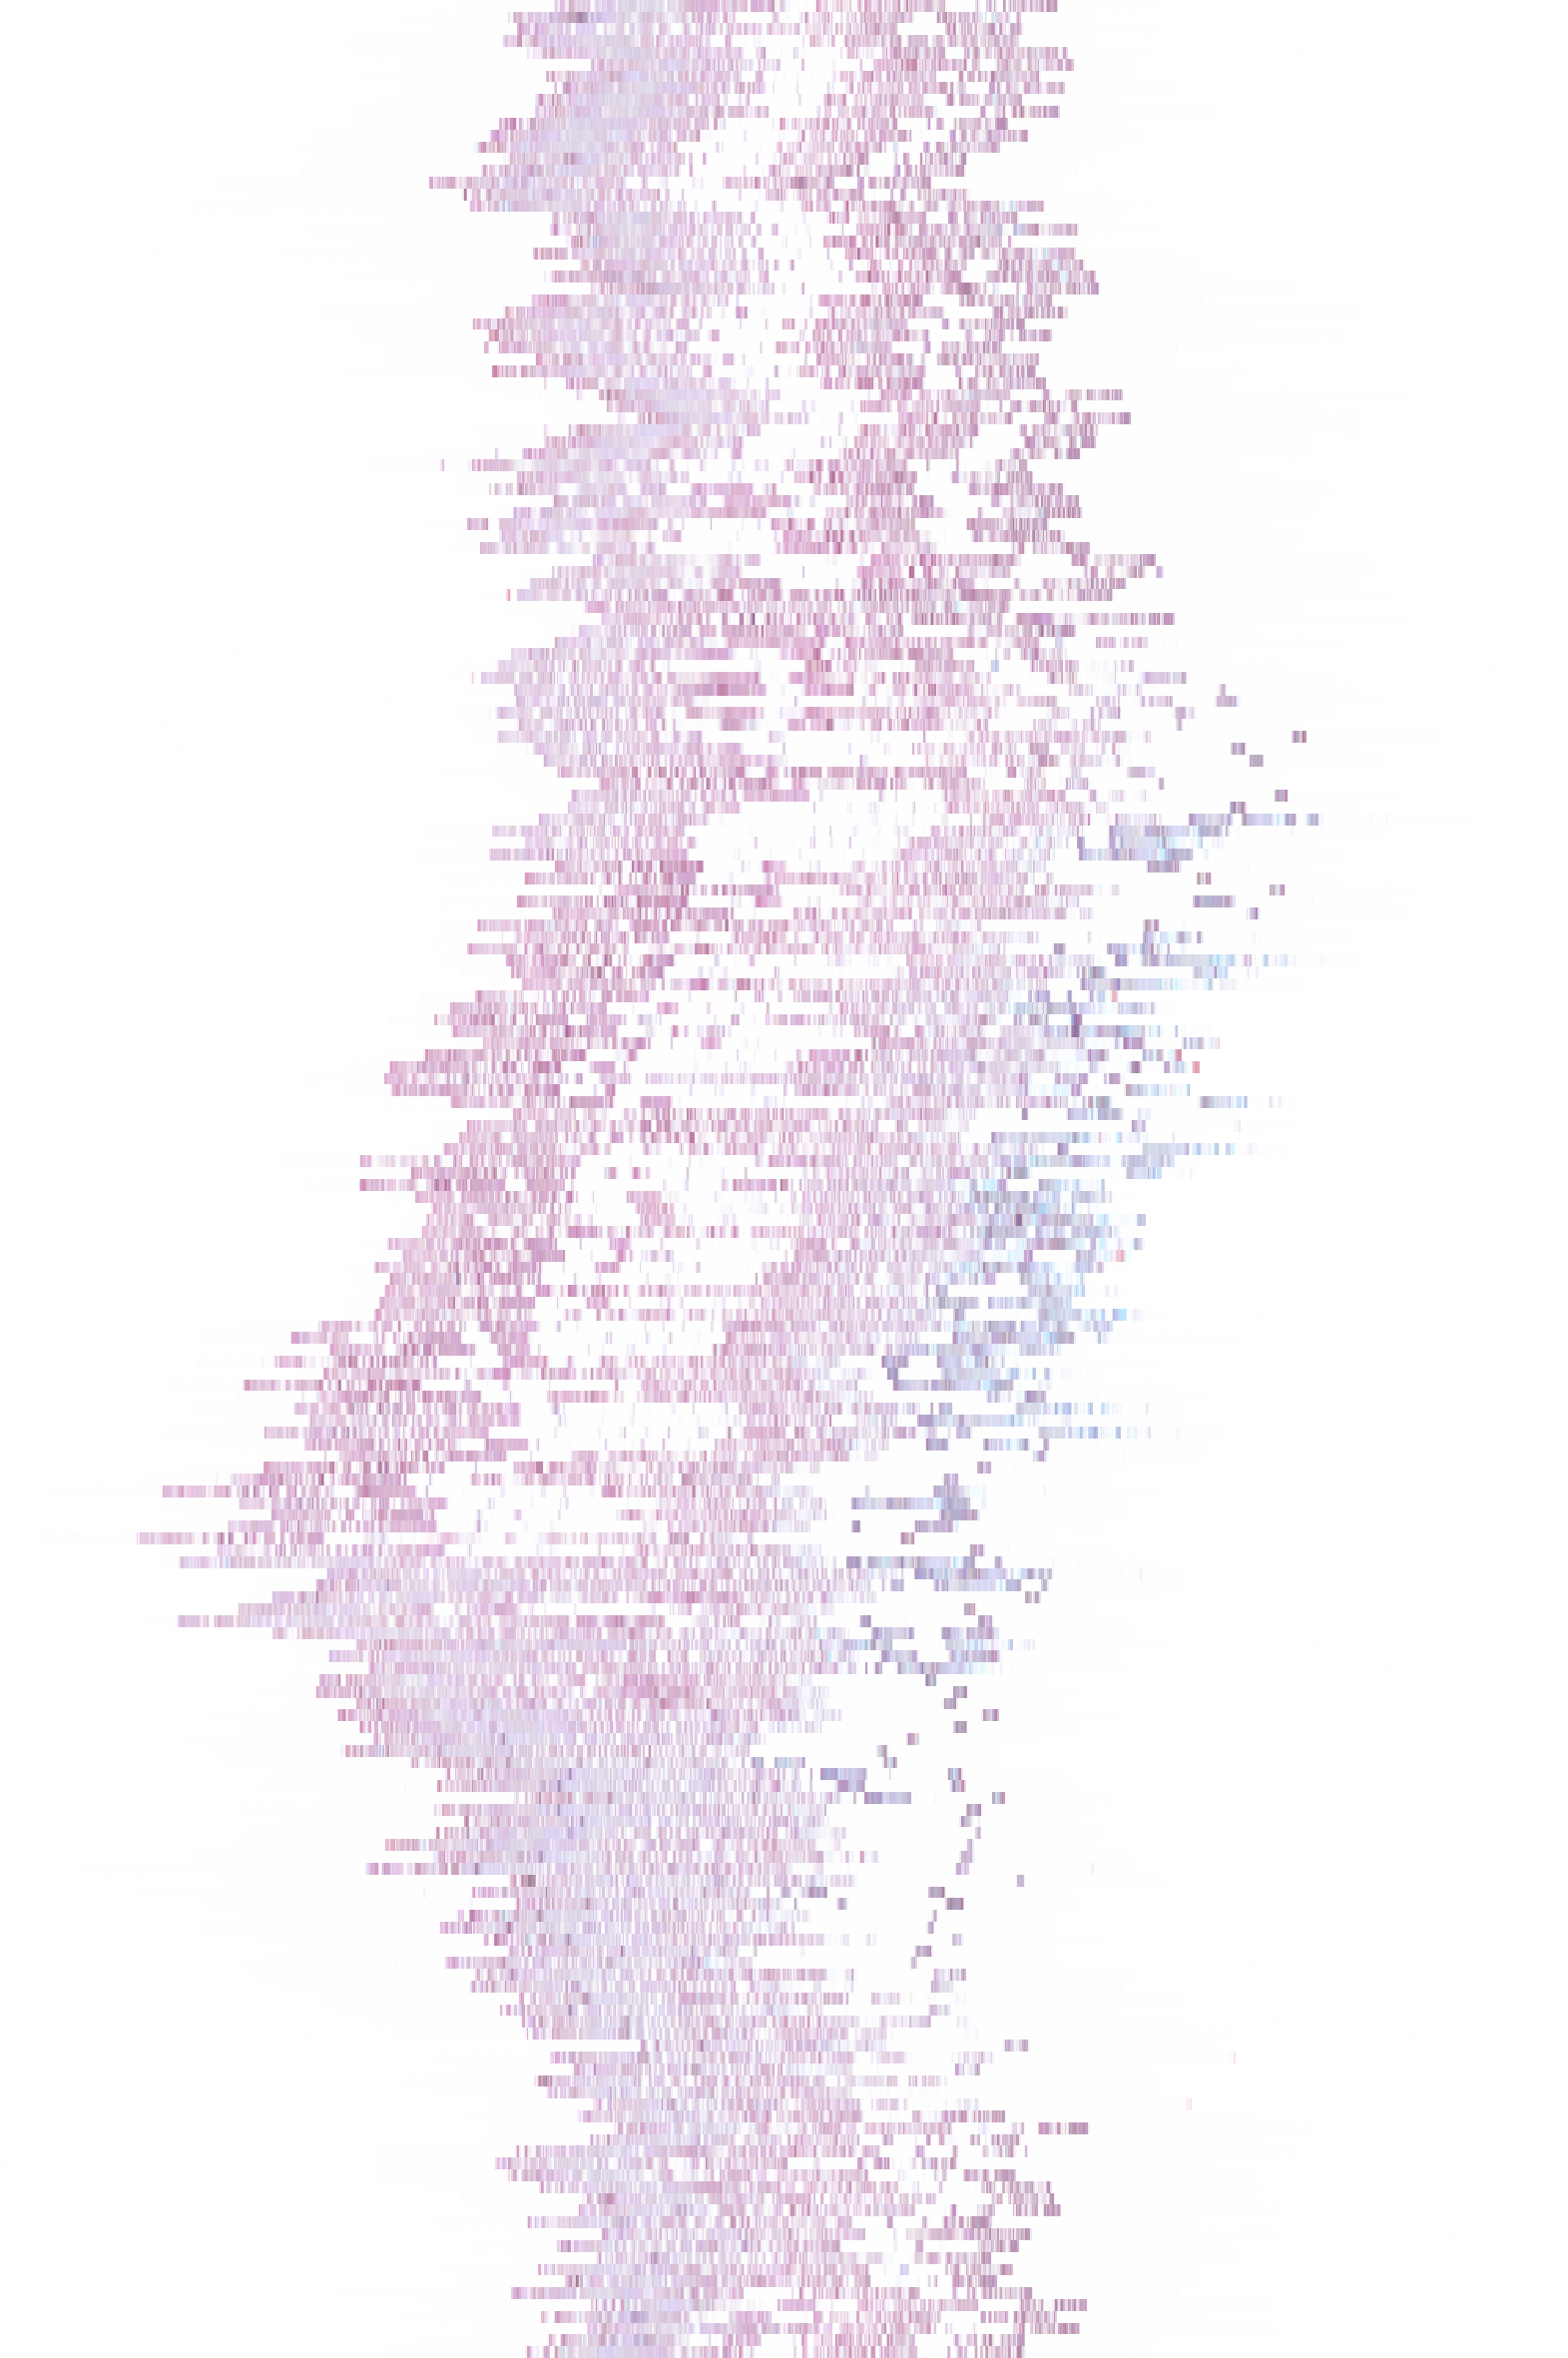
\includegraphics[width=1.1in]{2_methods/Figs/cross_section_1}}
    \subfloat[]{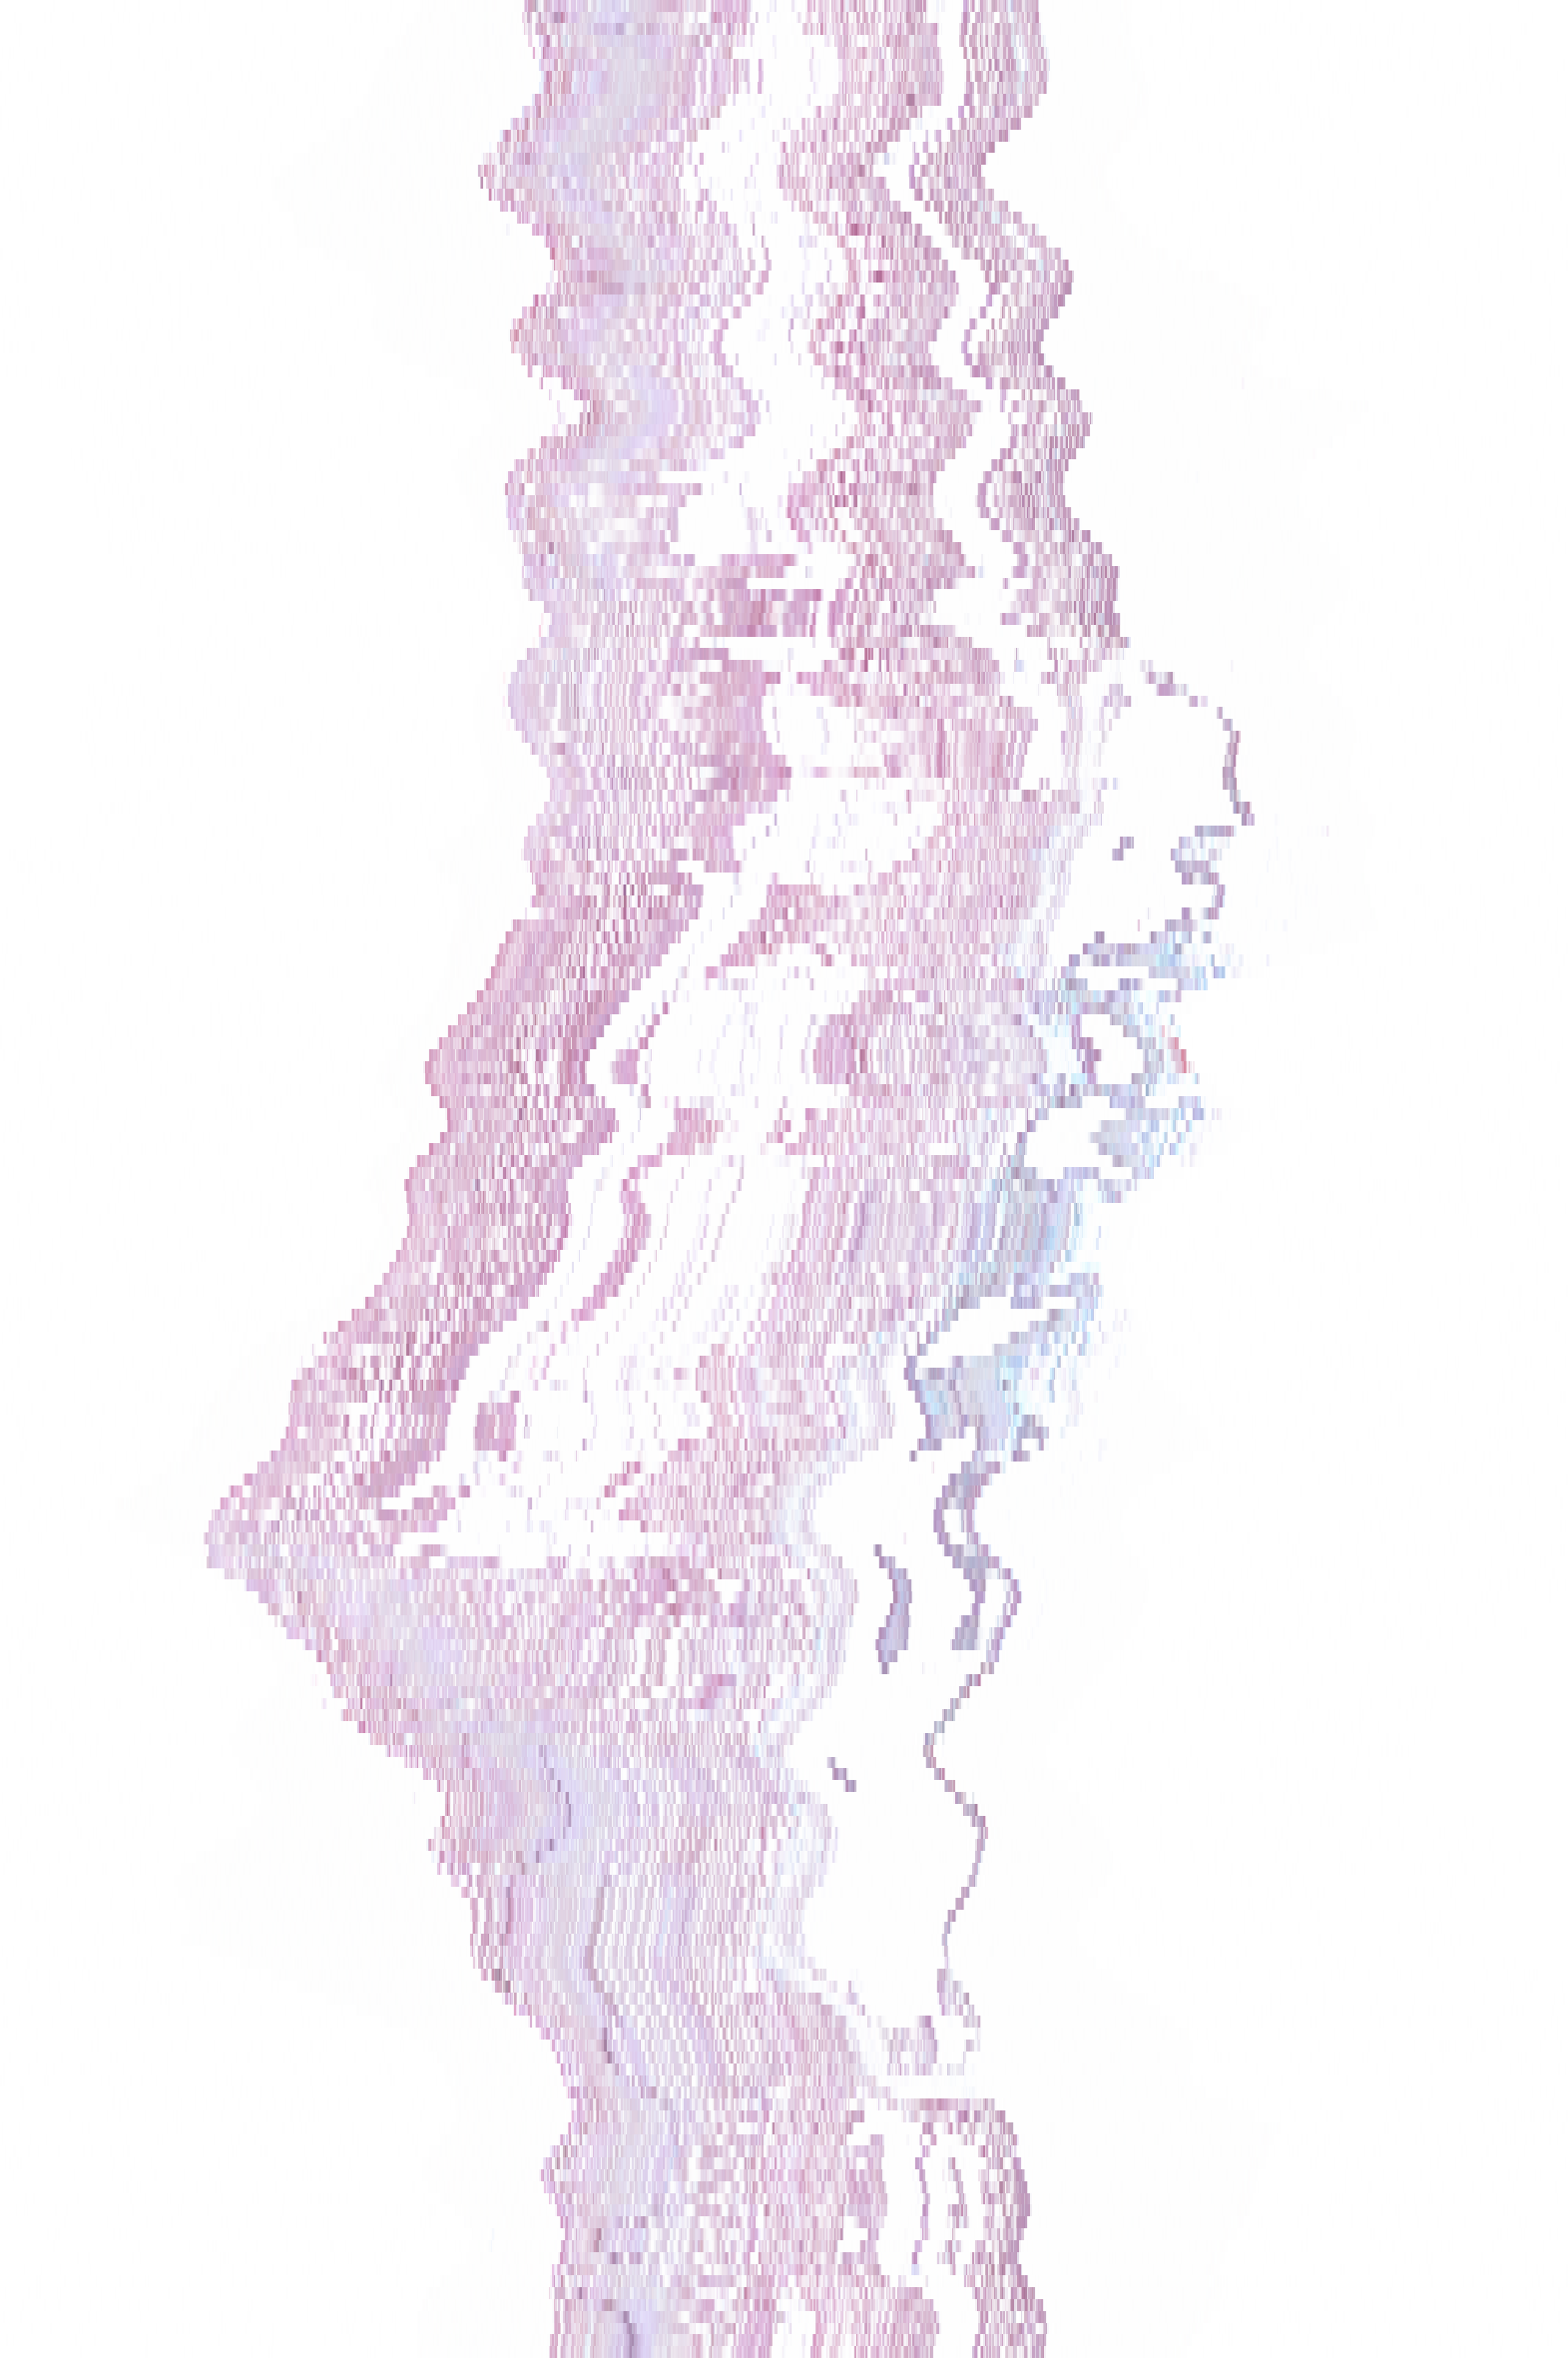
\includegraphics[width=1.1in]{2_methods/Figs/cross_section_7}}\\
    \subfloat[]{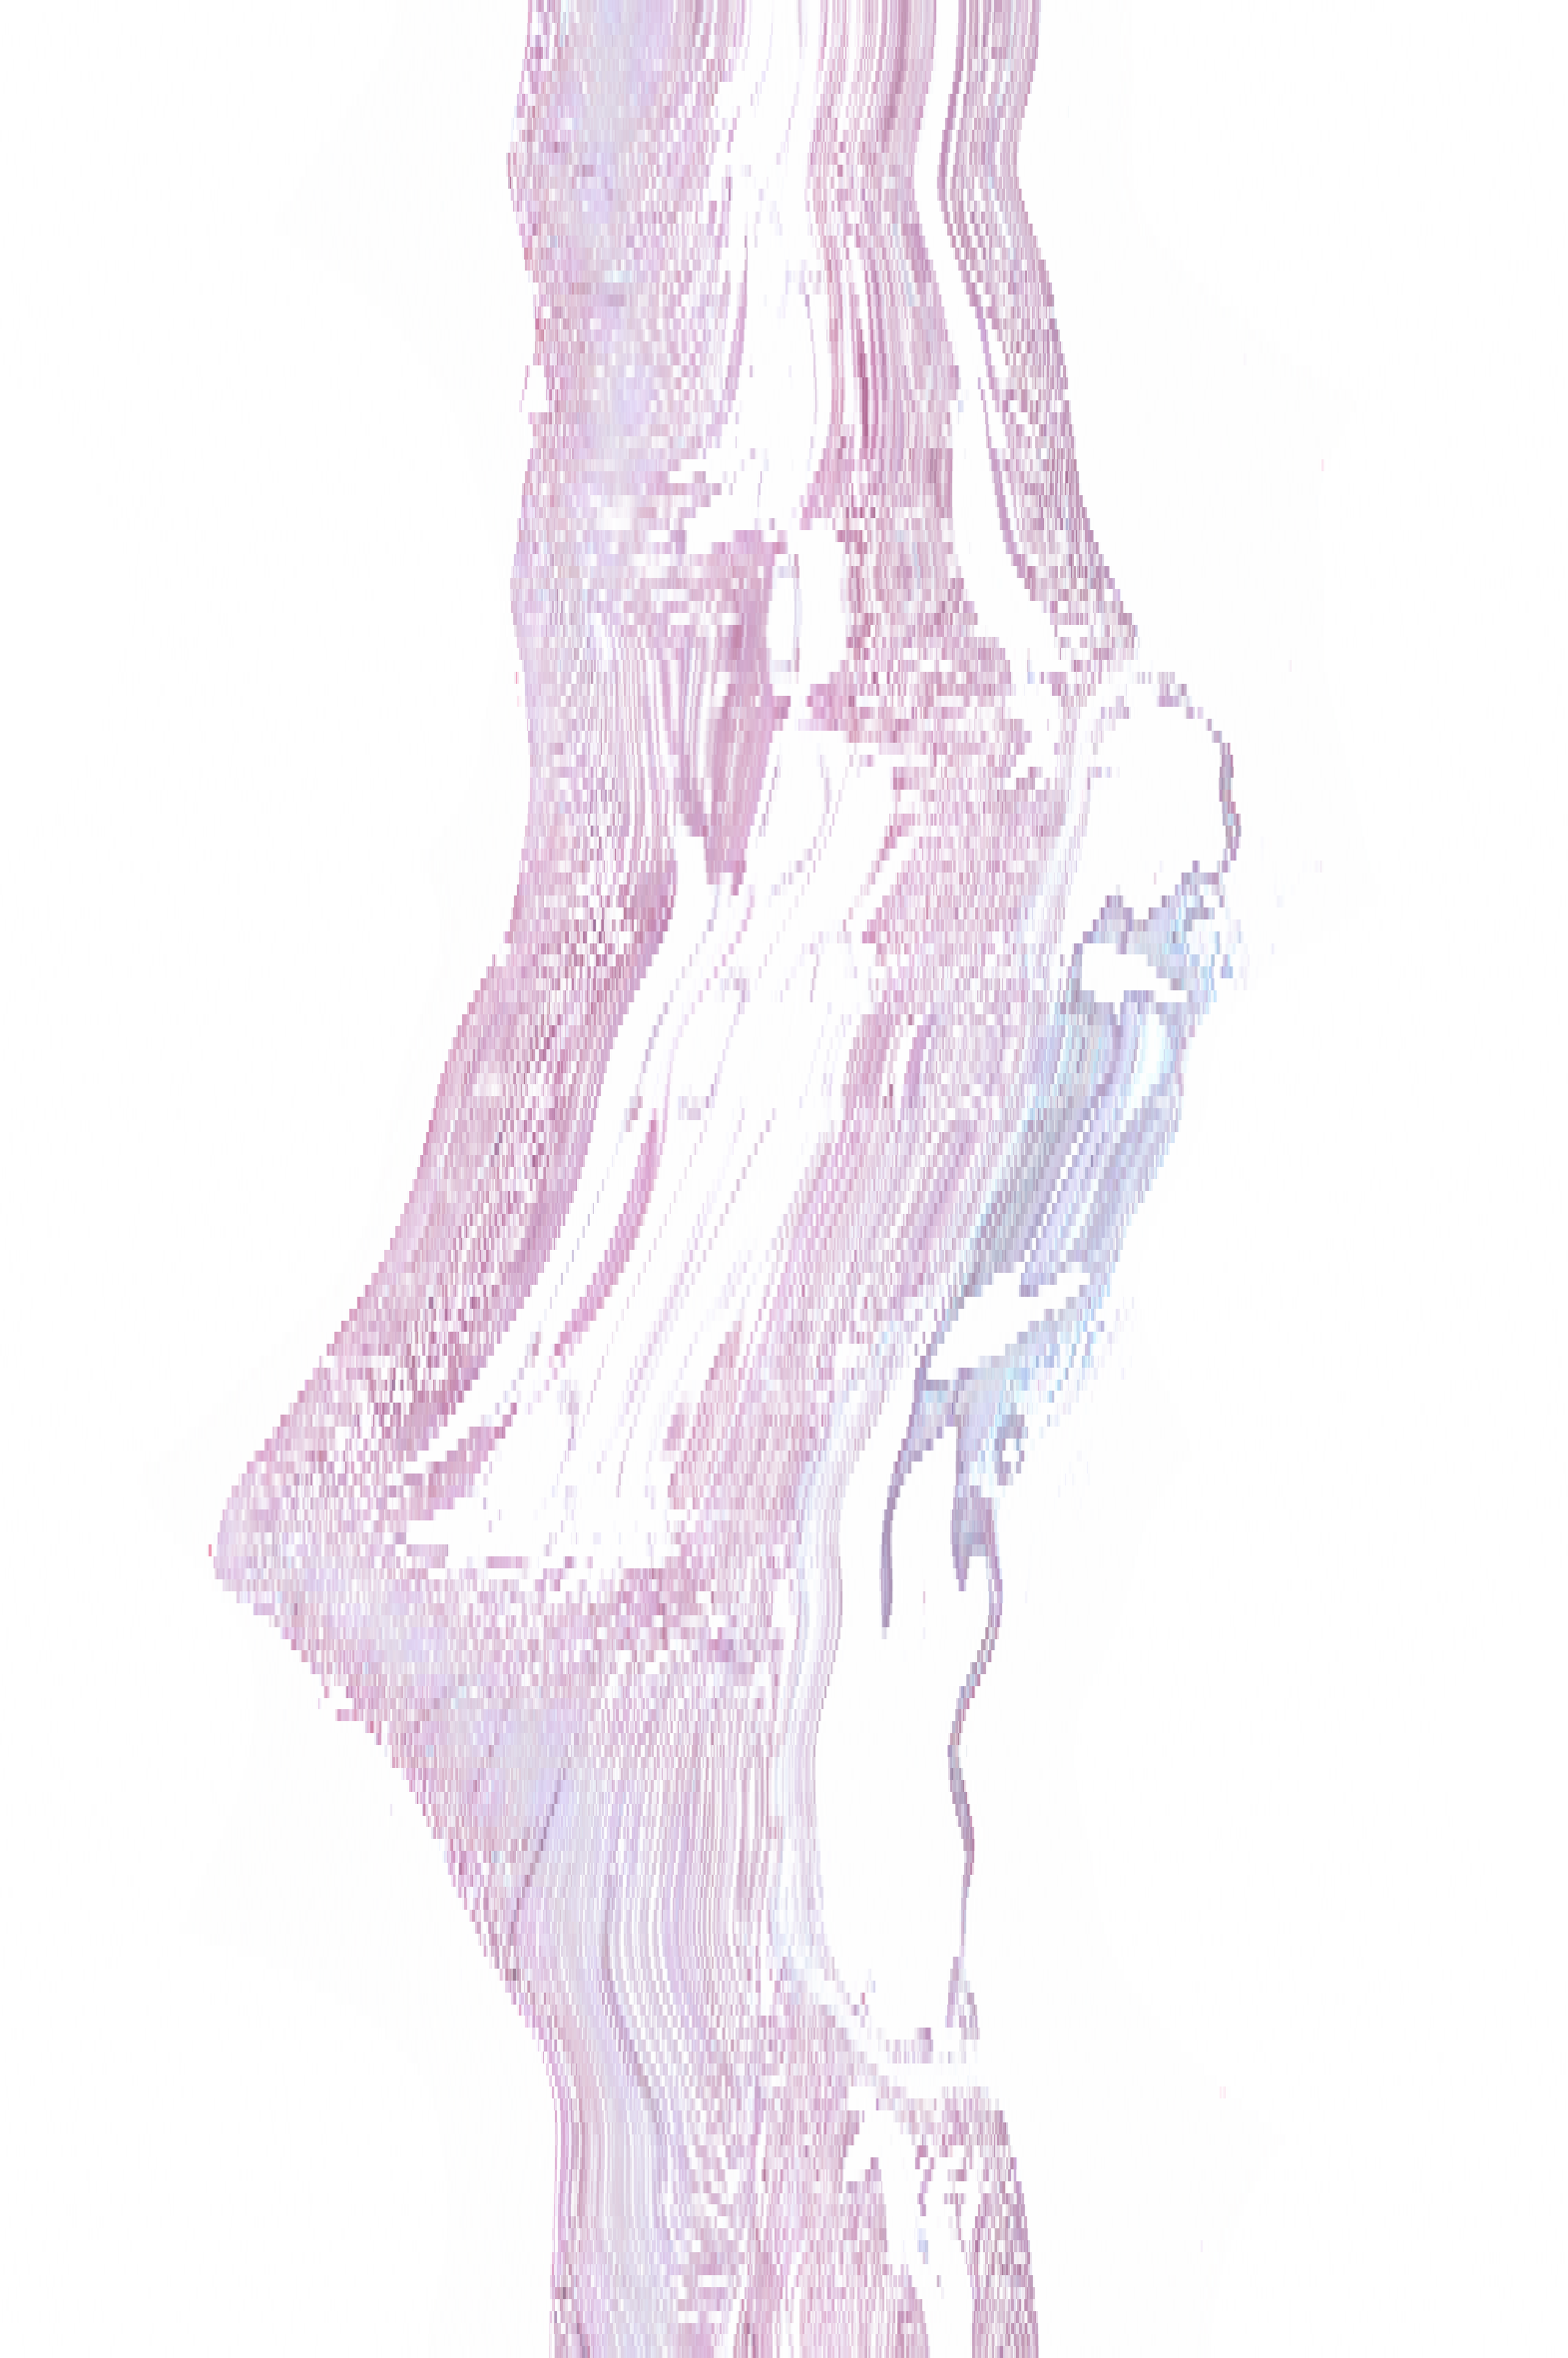
\includegraphics[width=1.1in]{2_methods/Figs/cross_section_40}}
    \subfloat[]{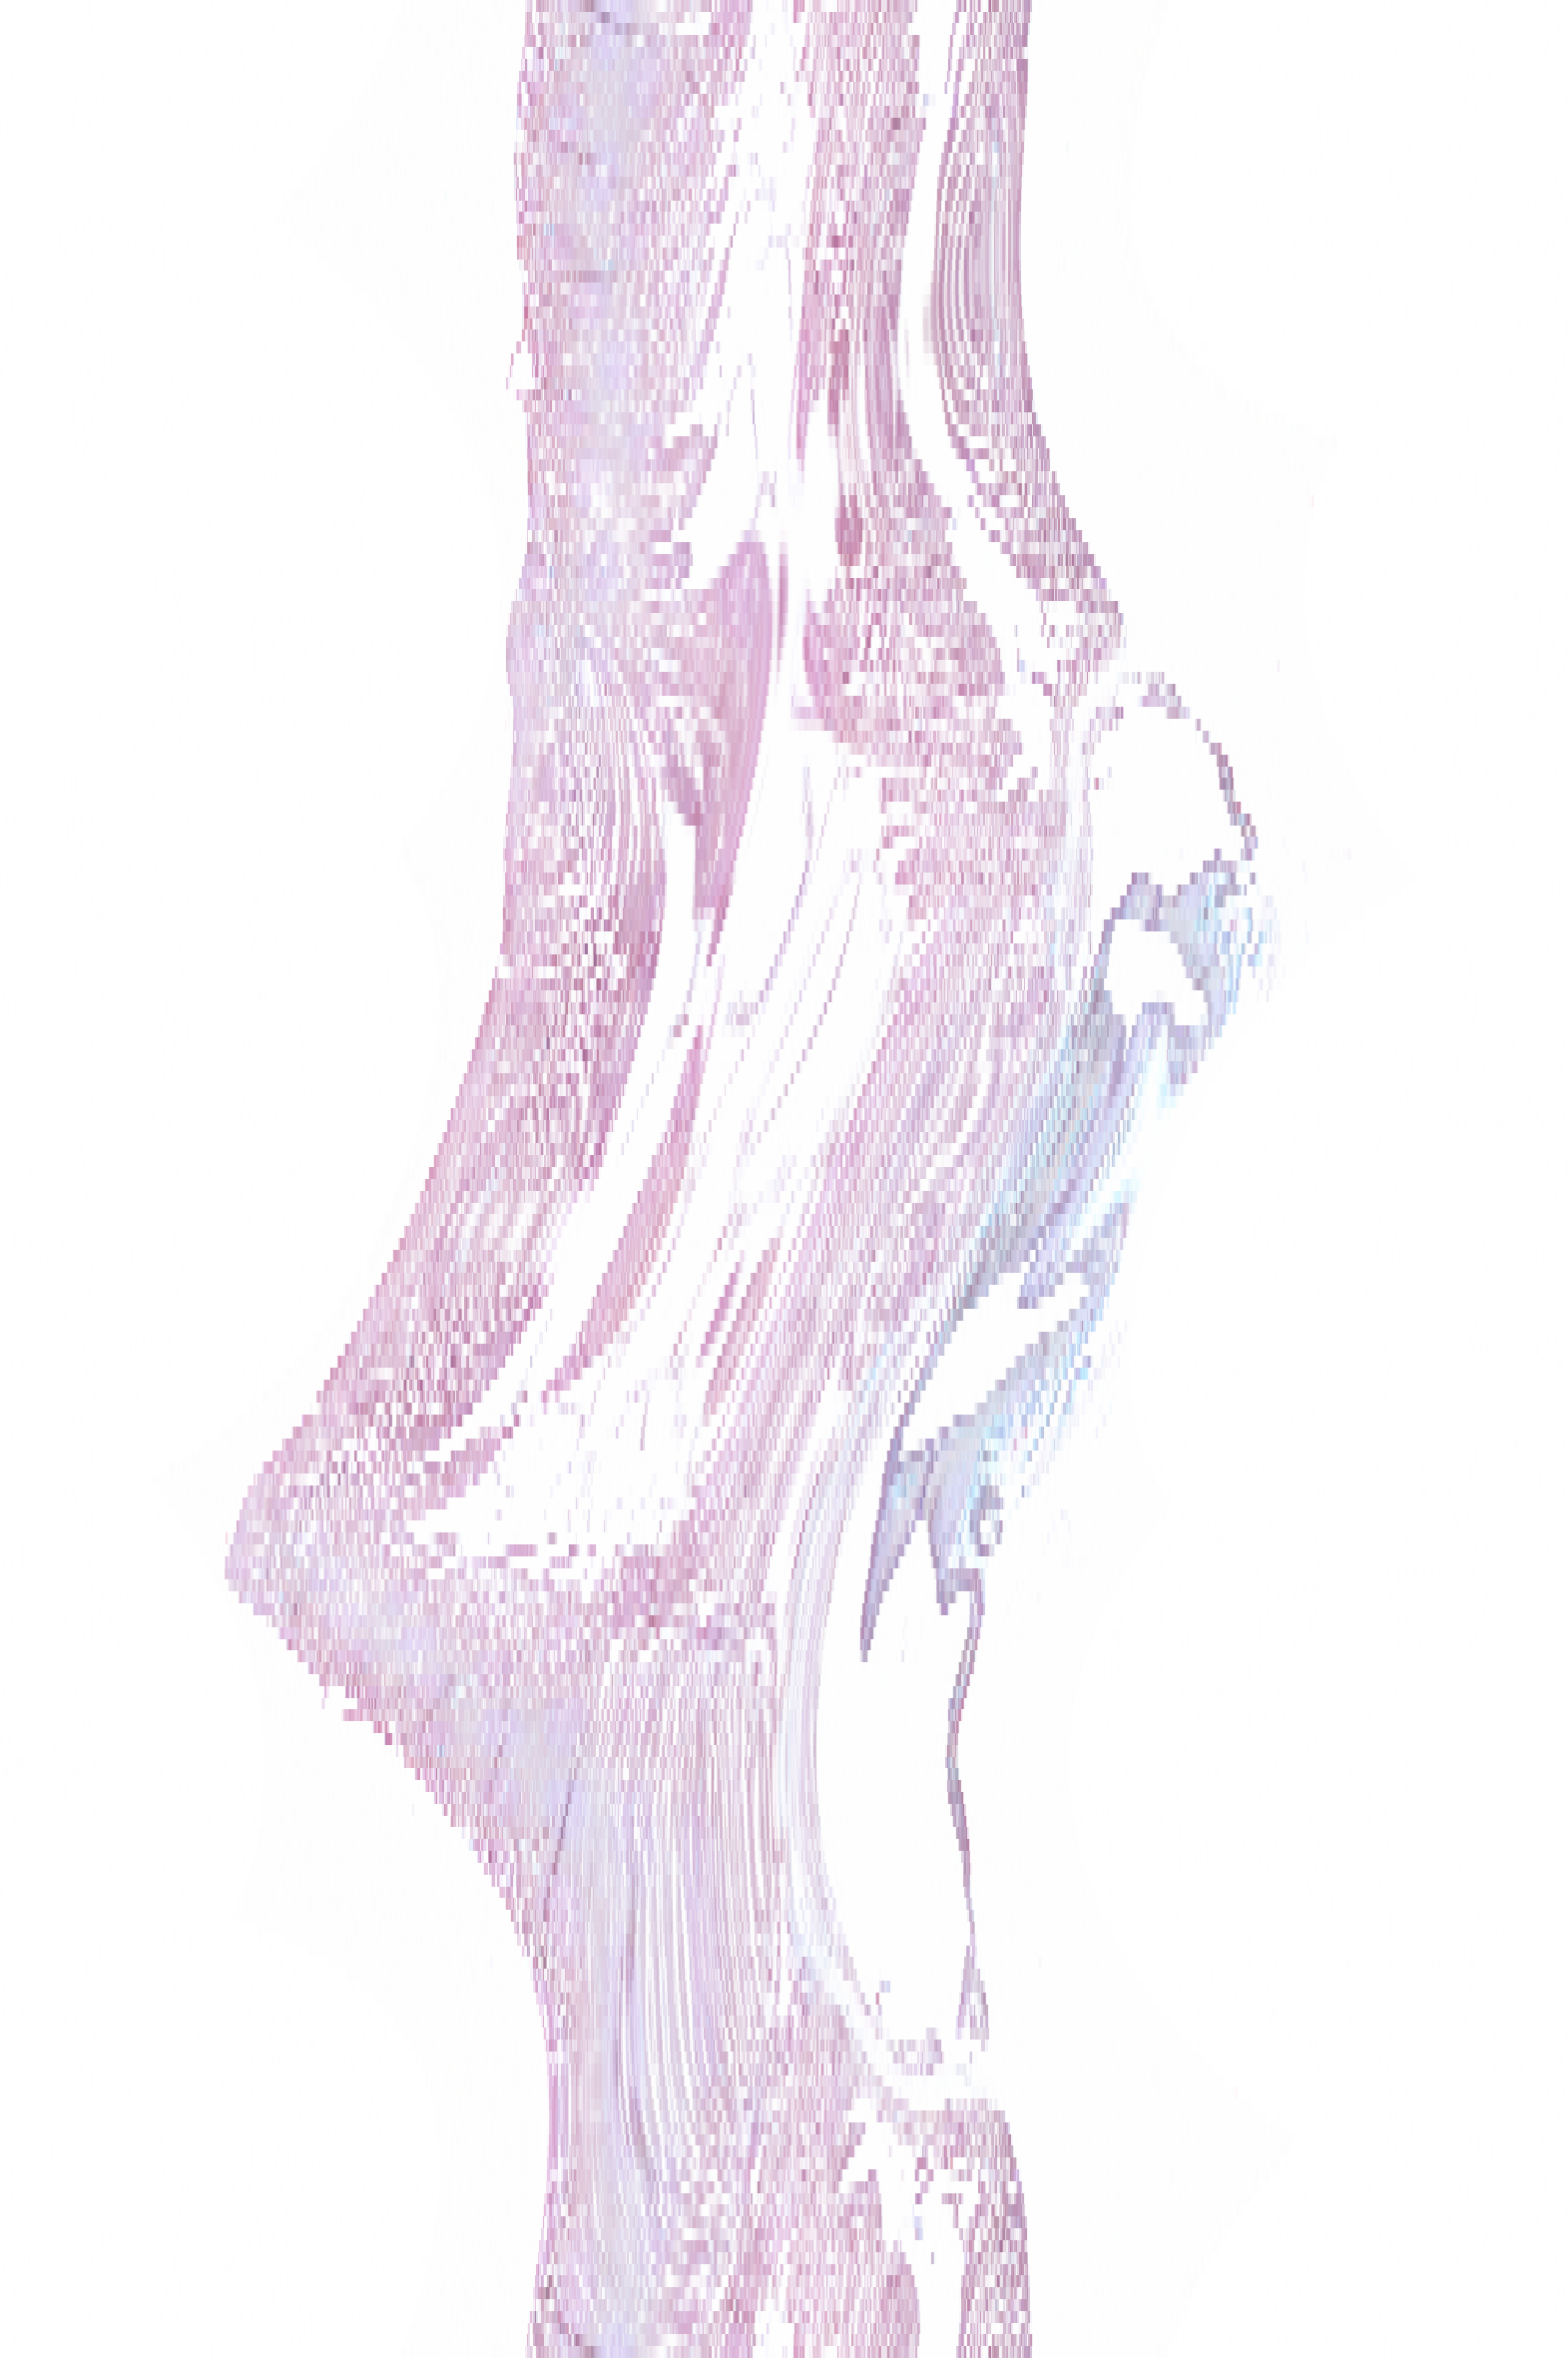
\includegraphics[width=1.1in]{2_methods/Figs/cross_section_perfect}}
    \subfloat[]{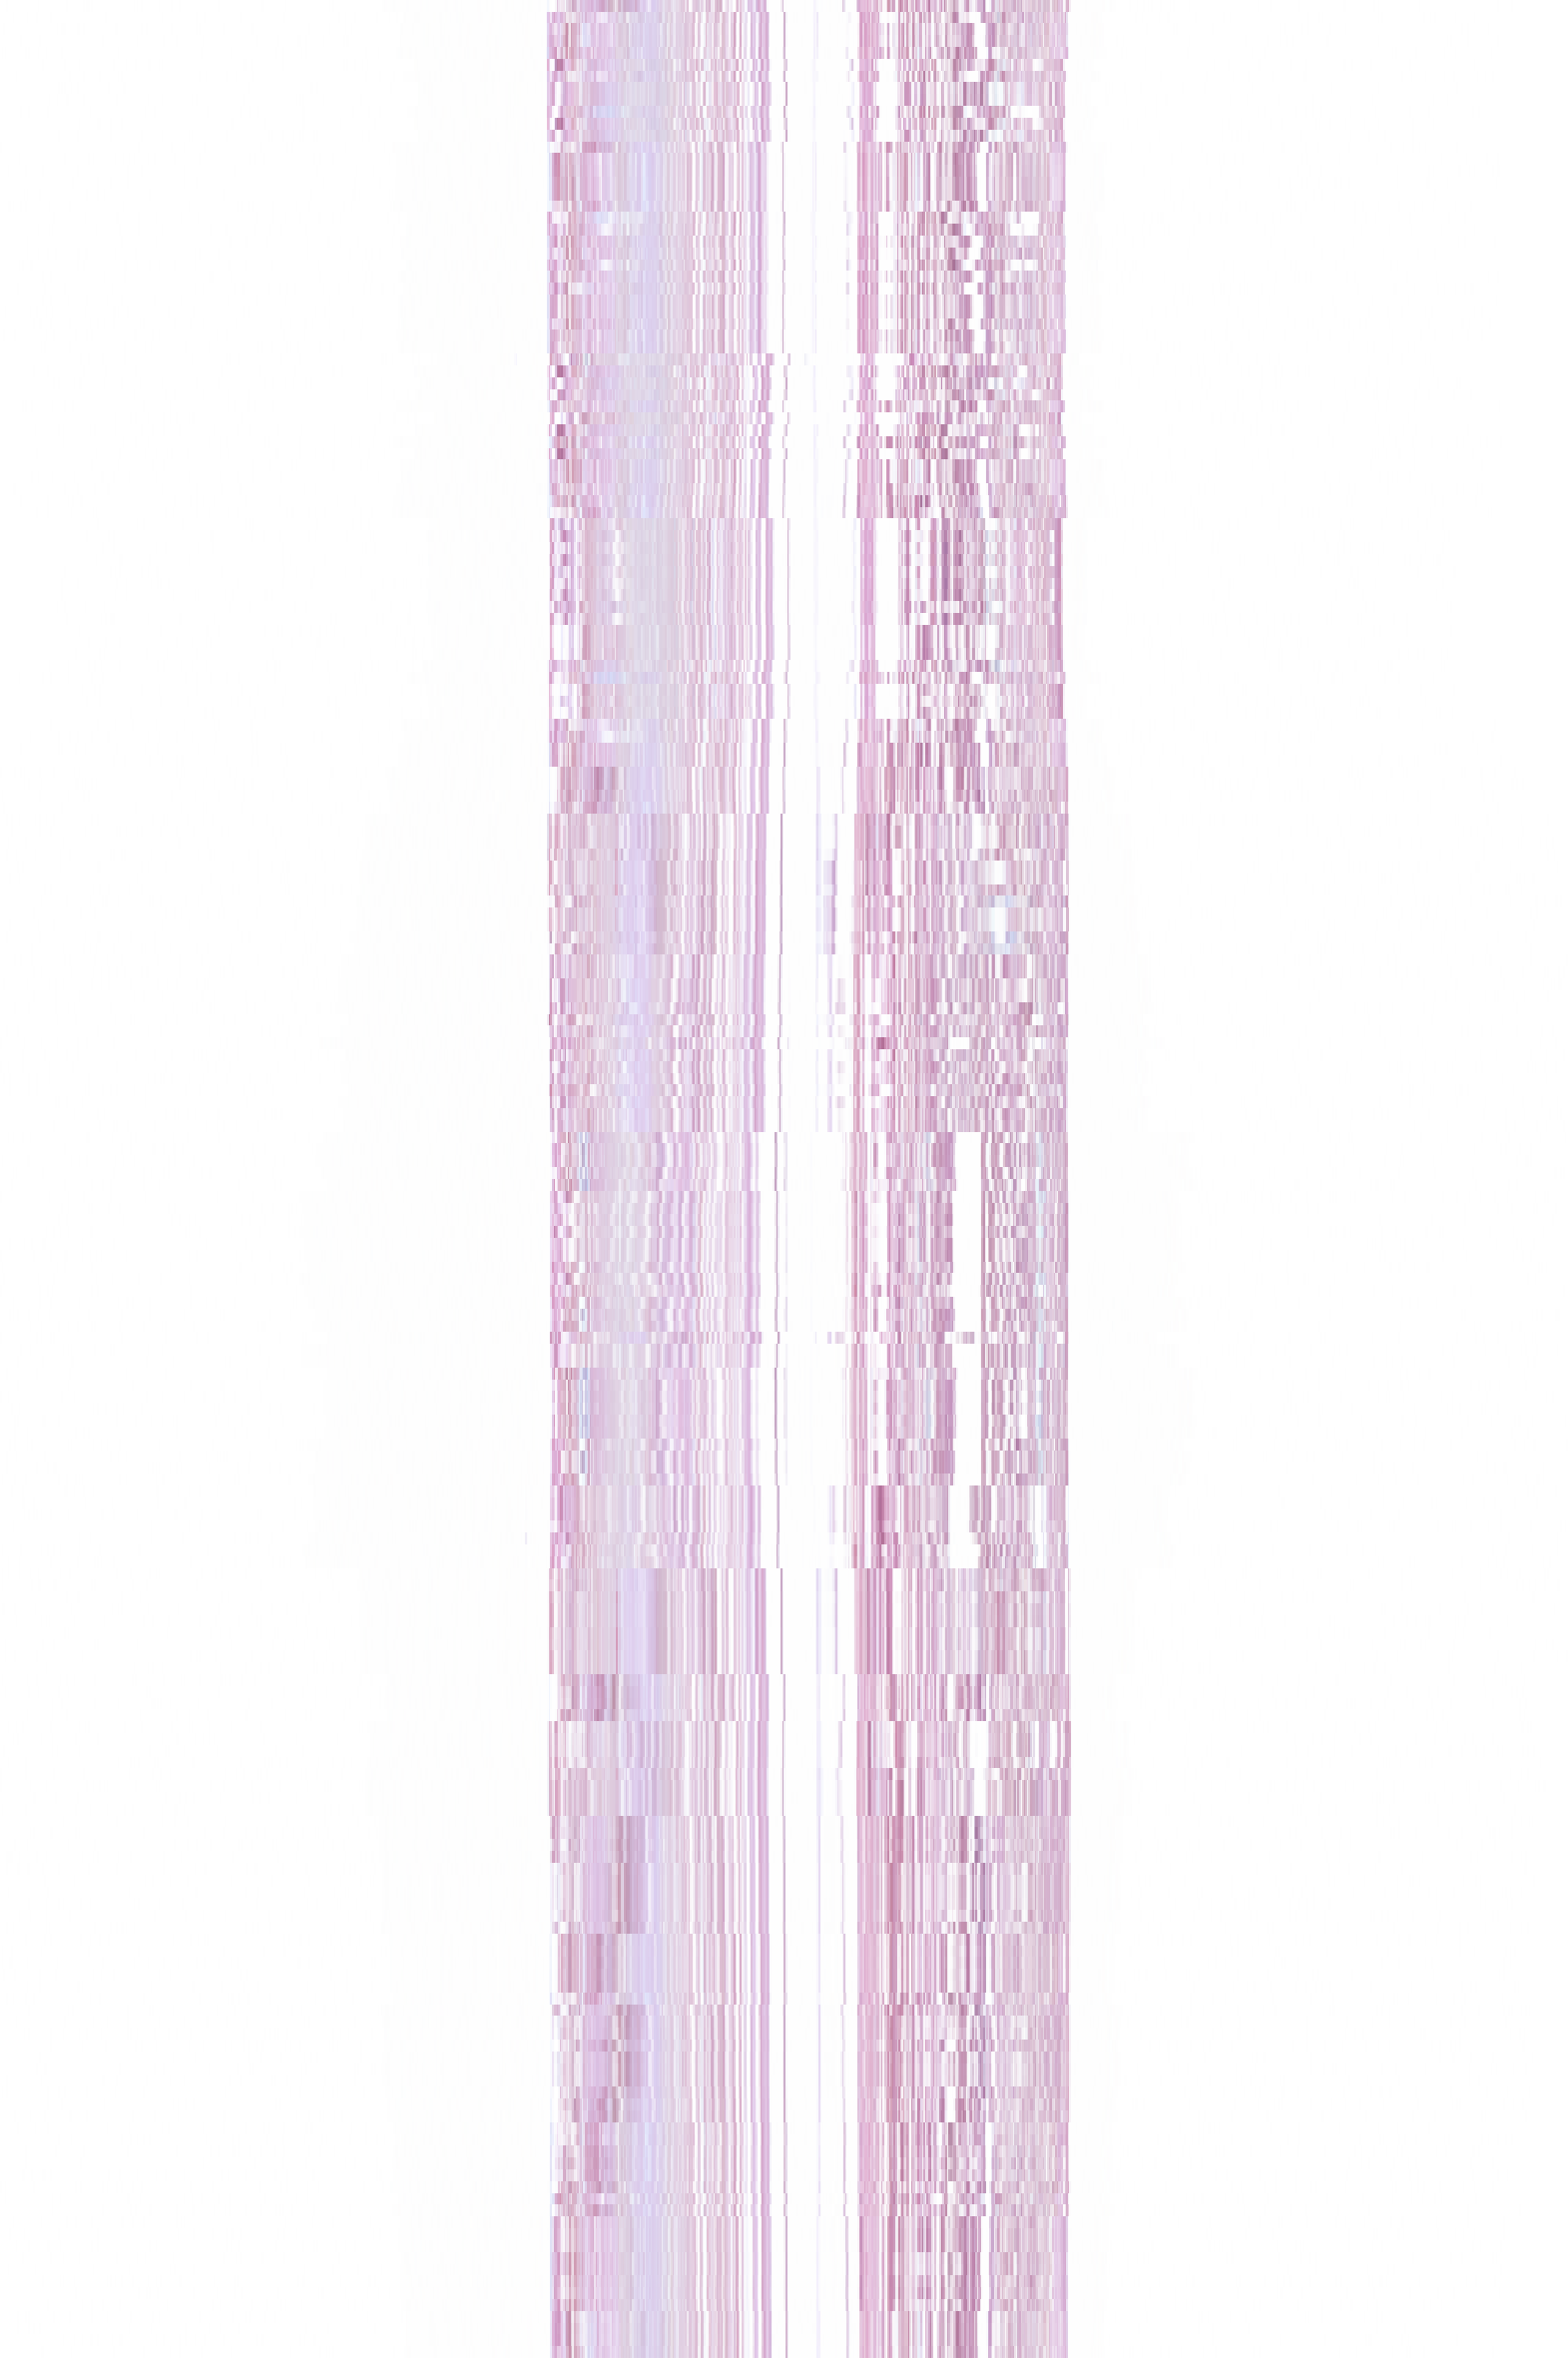
\includegraphics[width=1.1in]{2_methods/Figs/cross_section_banana}}
    \caption{Cross-sections of the synthetic volume (a) before TDS, (b) after 1 iteration, (c) after 7 iterations and (d) after 40 iterations, with (e) a cross-section of the unperturbed volume as a reference. (f) is the cross-section of a volume after serial slice-to-slice registration, where the straightening of the reconstruction resulting from the aforementioned 'banana effect' is evident.}
    \label{fig:synthetic_cross_sections}
  \end{figure}
  The central cross-sections of the synthetic geometries perpendicular to the x-axes are exhibited in Figure~\ref{fig:synthetic_cross_sections}. Cross-section (a) is of the original unsmoothed noisy volume. Cross-section (e) depicts the volume before noise is added; this volume is used as a ground truth to evaluate the effectiveness of TDS at removing high-frequency slice-to-slice misalignments. Three images are sandwiched by these two extremes, of sections smoothed 1, 7 and 40 times. Visually, the smoothing appears to perform well on two fronts. By iteration 40, a smooth, continuous section with the appearance of an original histology slice has been recovered from an unrecognisably noisy volume. Secondly and crucially, the underlying geometry of the tissue has been preserved, as can be seen by comparison to the ground truth sections in (e). To illustrate the banana effect, we performed a slice-to-slice registration in which each slice is aligned to that immediately below. The resulting structure, shown in (f), has lost virtually all of the underlying ground truth shape.
  
  \begin{figure}[!t]
    \centering
    \subfloat[]{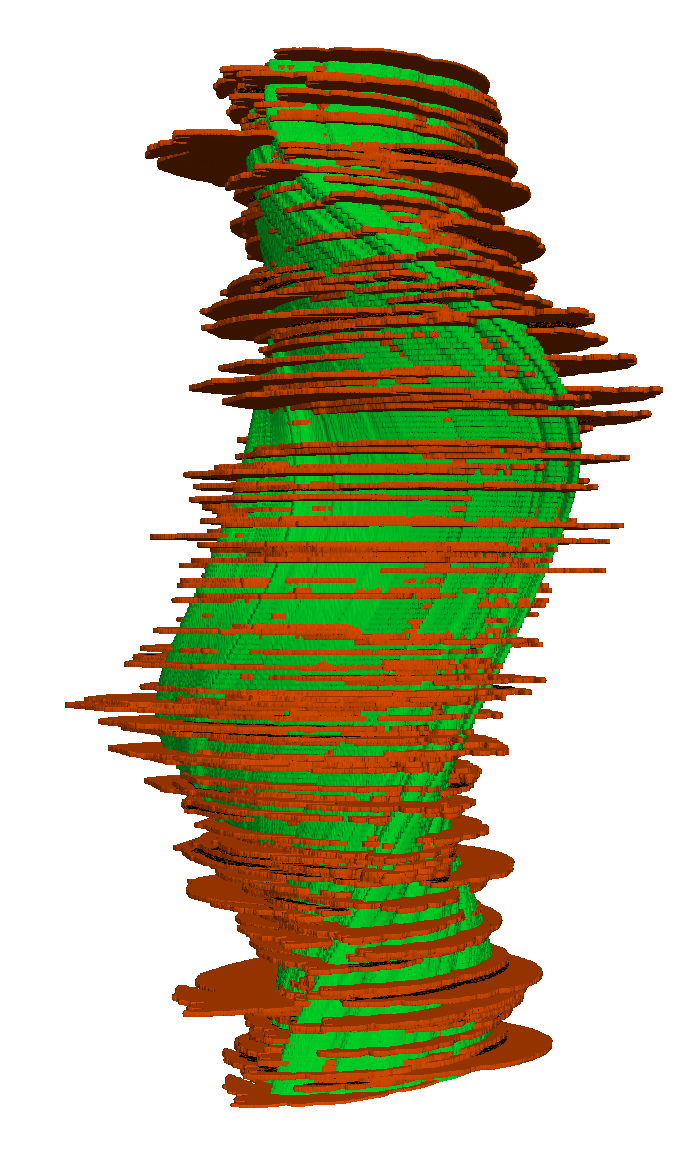
\includegraphics[width=1.1in]{2_methods/Figs/whole_surface_0}}
    \subfloat[]{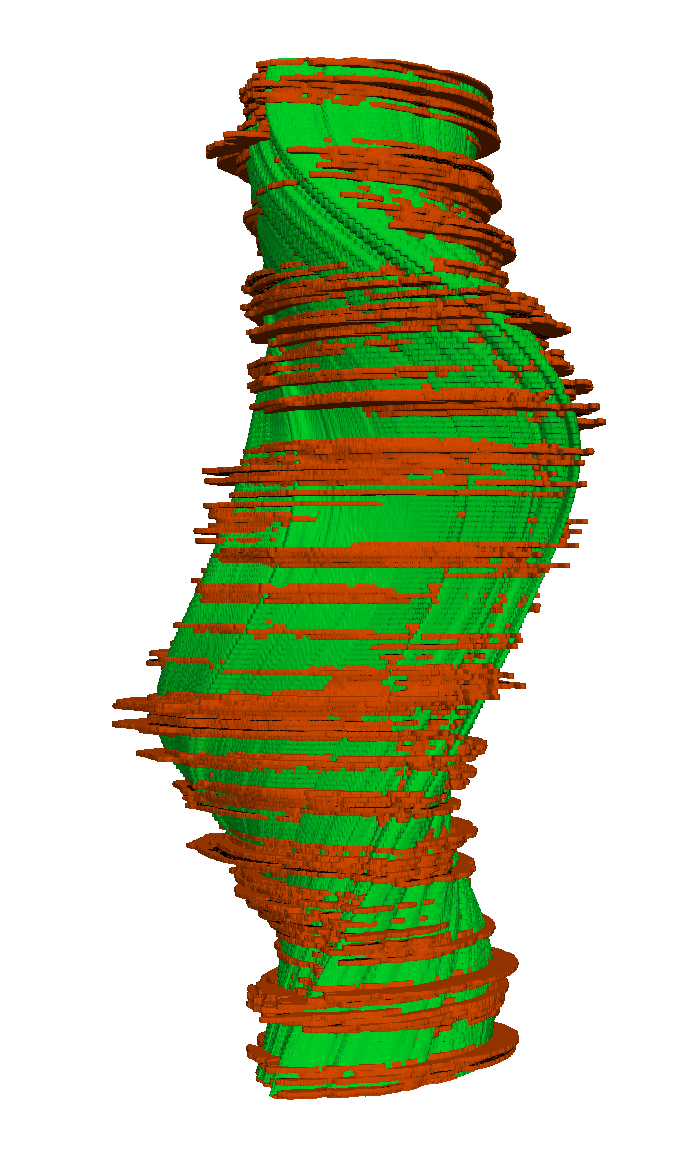
\includegraphics[width=1.1in]{2_methods/Figs/whole_surface_1}}
    \subfloat[]{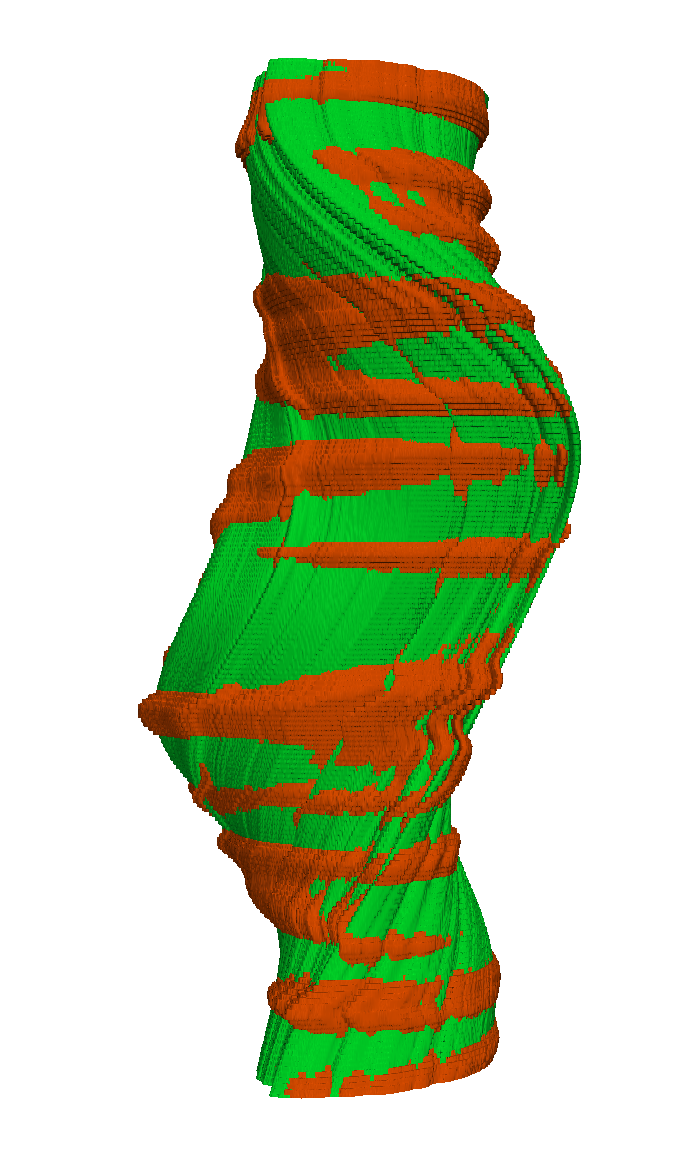
\includegraphics[width=1.1in]{2_methods/Figs/whole_surface_7}}\\
    \subfloat[]{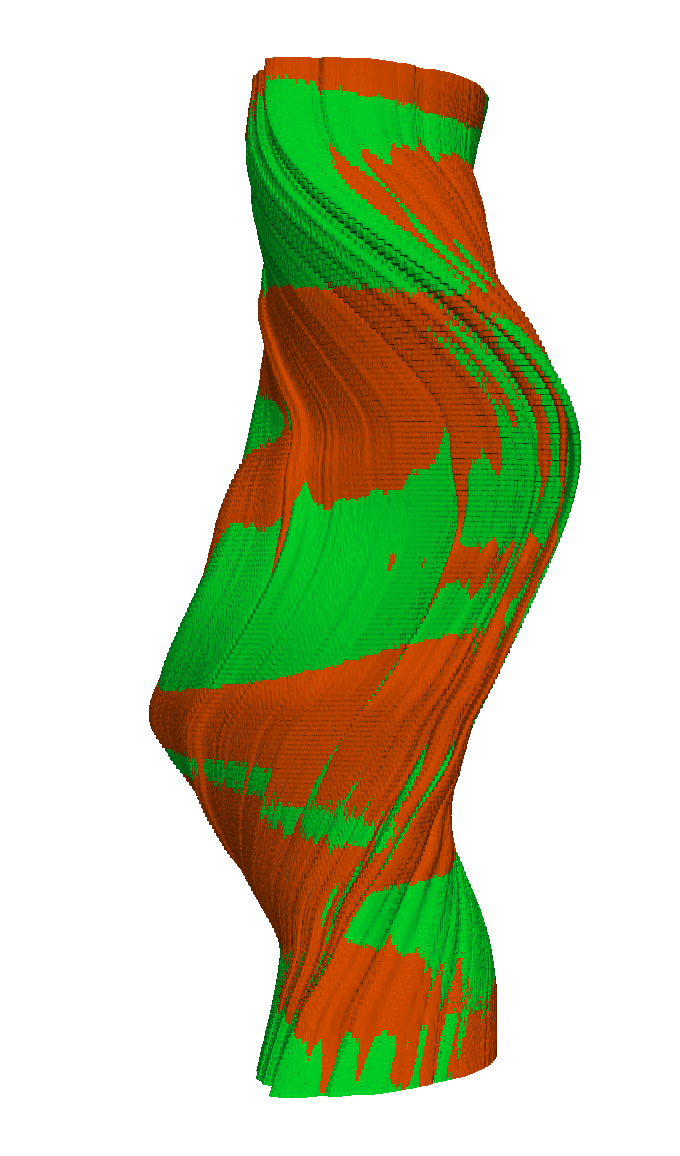
\includegraphics[width=1.1in]{2_methods/Figs/whole_surface_40}}
    \subfloat[]{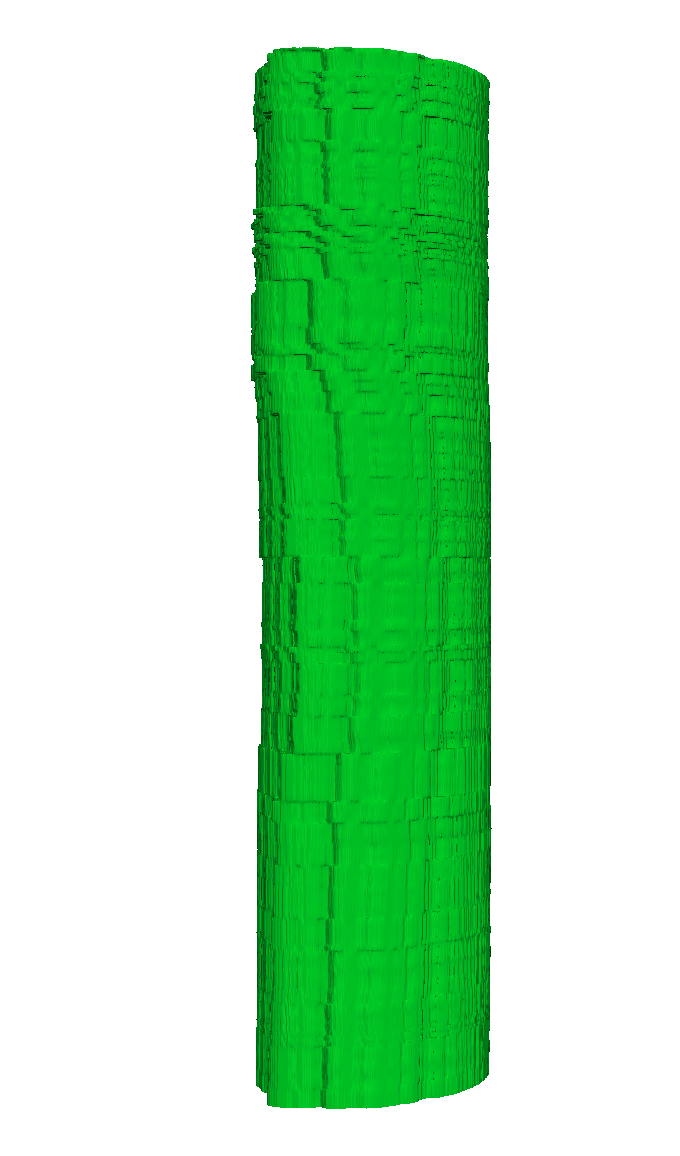
\includegraphics[width=1.1in]{2_methods/Figs/whole_surface_banana}}
    \caption{The same results of Figure 2, here shown as contours in a 3D representation. The synthetic volumes are shown in red before TDS (a), and after 1 (b), 7 (c) and 40 (d) iterations, overlayed with the unperturbed volume in green. A contour of the serially registered volume is shown in green in (e), again clearly illustrating the banana effect.}
    \label{fig:synthetic_contours}
  \end{figure}
  The nature of the 3-D geometry of the volumes --- the rotation and translation signals and the transformational noise --- is most clearly understood from the segmentation volume isosurfaces in Figure~\ref{fig:synthetic_contours}. Each of the 4 levels of smoothing depicted by Figure~\ref{fig:synthetic_cross_sections} are overlayed in red with the unperturbed volume in green. Again, the smoothing brings the noisy volume closely in line with the ground truth, with the largest effect on the higher frequencies of noise. The conservation of the underlying structure is most evident in Figure~\ref{fig:synthetic_contours}~(d), where the red isosurface deviates almost imperceptibly from the green. Apart from the obvious straightening of the volume, the surface of (e) is greatly more discontinous than the red surface of (d), each slice pair having only been coregistered once.

  % Evolution of error from ground truth
  \begin{figure}[!t]
    \subfloat[]{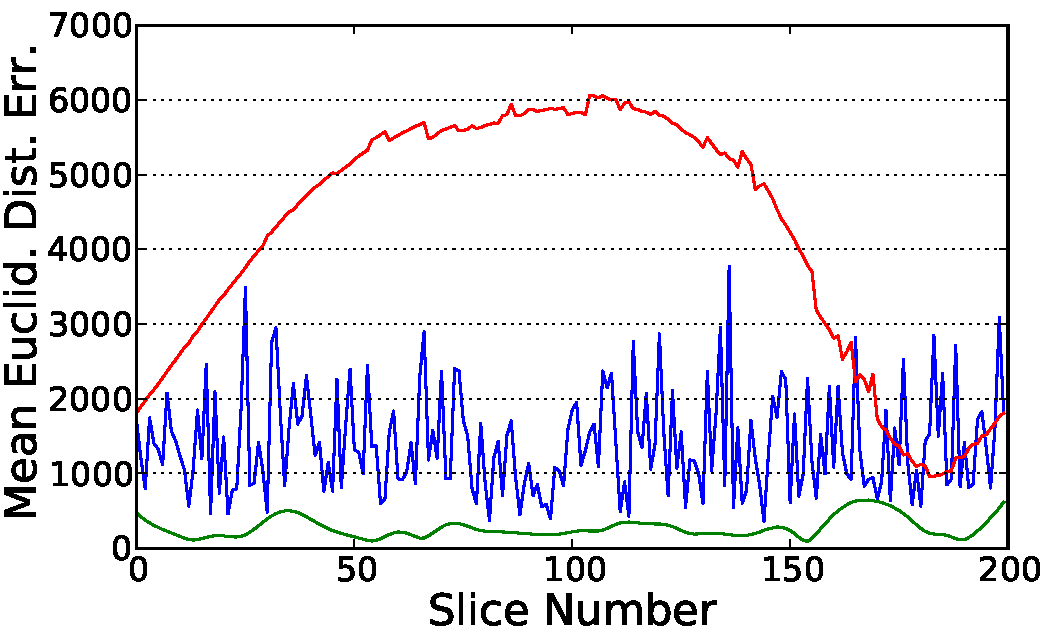
\includegraphics[width=1.7in]{2_methods/Figs/absolute_errors_2d}\label{fig:absolute_errors_2d}}
    \subfloat[]{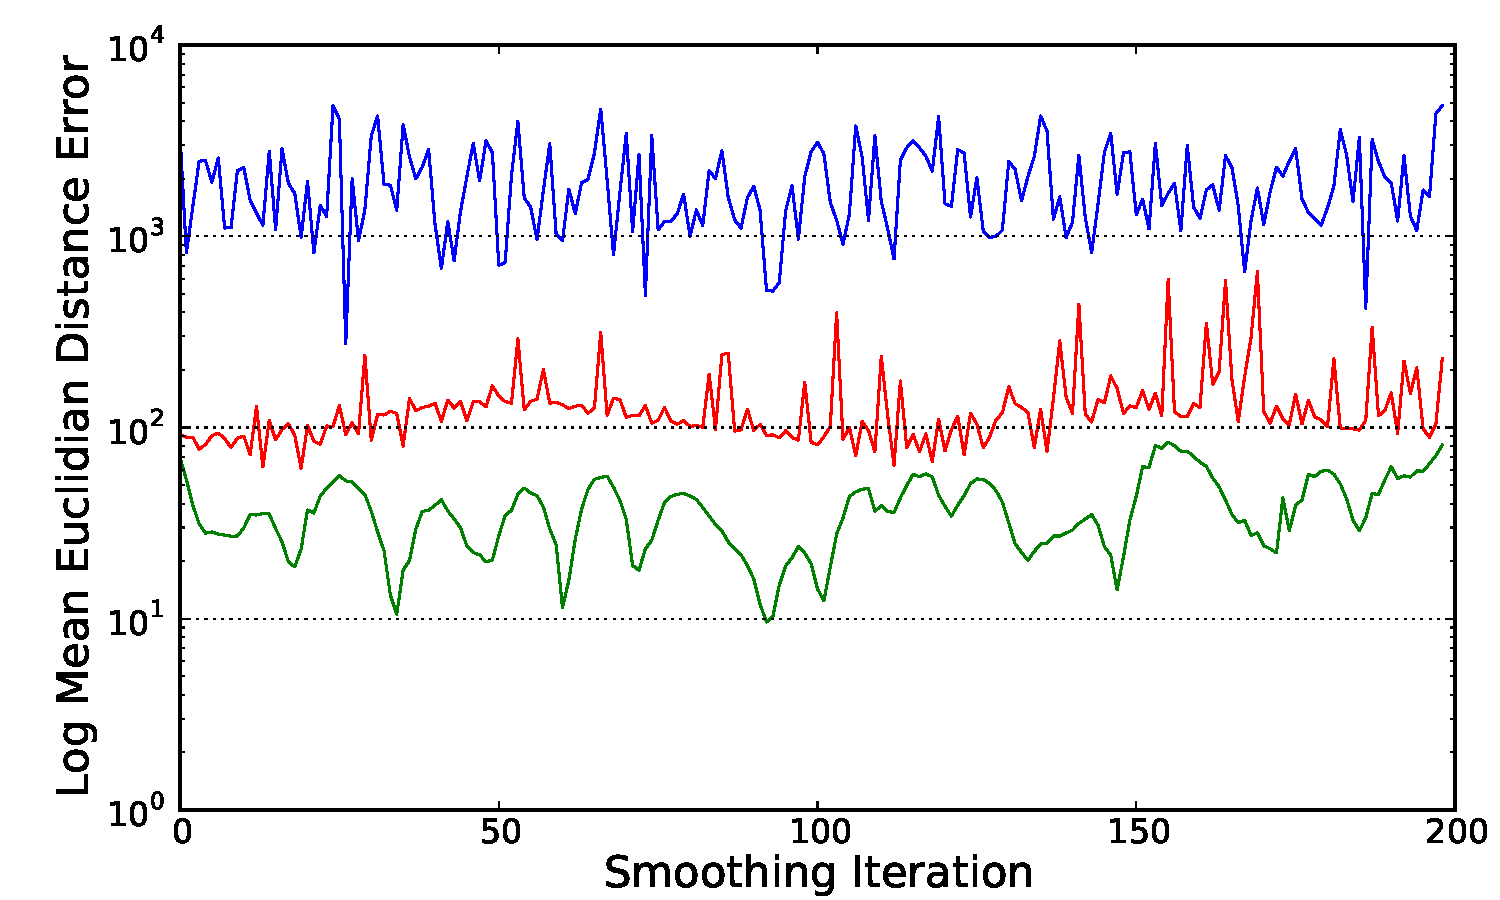
\includegraphics[width=1.7in]{2_methods/Figs/relative_errors_2d}\label{fig:relative_errors_2d}}
    \caption{Slicewise absolute (a) and relative (b) mean pixel Euclidean distance errors of the initial (before TDS, blue), final (after TDS, green) and sequentially registered (red) synthetic volumes. The absolute volumewise distance means are 1393, 271.6 and 4204 and the relative means are 1929, 37.94 and 134.8, for the initial, final and sequential volumes respectively.}
    \label{fig:synthetic_errors}
  \end{figure}
  Figure~\ref{fig:synthetic_errors} shows a quantitative evaluation of the fidelity of TDS reconstructed results to the original dataset. The slices were first segmented to separate tissue and non-tissue pixels, and the Euclidean distance of each tissue pixel from its ground truth position was calculated, before and after TDS and after serial slice-to-slice registration. The metric is greatly reduced after TDS, evidence that each slice is much more closely aligned to its true position. The overall sinusoidal nature of the serial registration is of course due to the loss of the ground truth morphology. The error after TDS is clearly the smoothest of the three lines, reflecting the continuity of the volume and the preferential damping of the high frequency spectrum.

  Mean relative Euclidean errors are also shown on a logarithmic scale in Figure~\ref{fig:synthetic_errors}~(b). These are defined as the distances of voxels in slice $n+1$ from their ground truth positions, both measured from the respective reference frames of slice $n$. The same spectral patterns are observed, with the sinusoidal pattern now removed by the relative calculation. Volumewise absolute error is reduced by a factor of 5.1 and relative error by 50 after TDS.

  \subsection{Block Face Registration of Histology} % (fold)
  \label{sub:block_face_registration_of_histology}
  % figure of full cross-sections, unregistered, banana registered and lo-res registered, with lores equivalent slice
  \begin{figure}[!t]
    \centering
    \subfloat[]{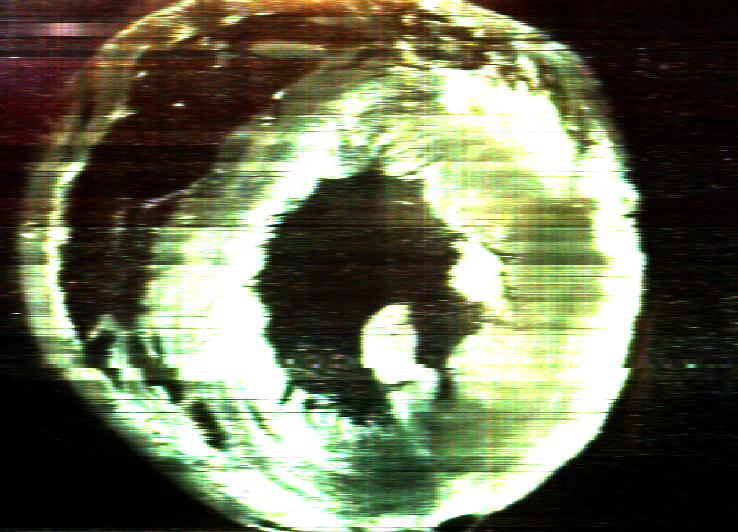
\includegraphics[height=1.2in]{3_results/Figs/LoRes_1_287}}
    \subfloat[]{
\includegraphics[height=1.2in]{3_results/Figs/geometric_1_287}}\\
    \subfloat[]{
\includegraphics[height=1.2in]{3_results/Figs/affine_1_287}}
    \subfloat[]{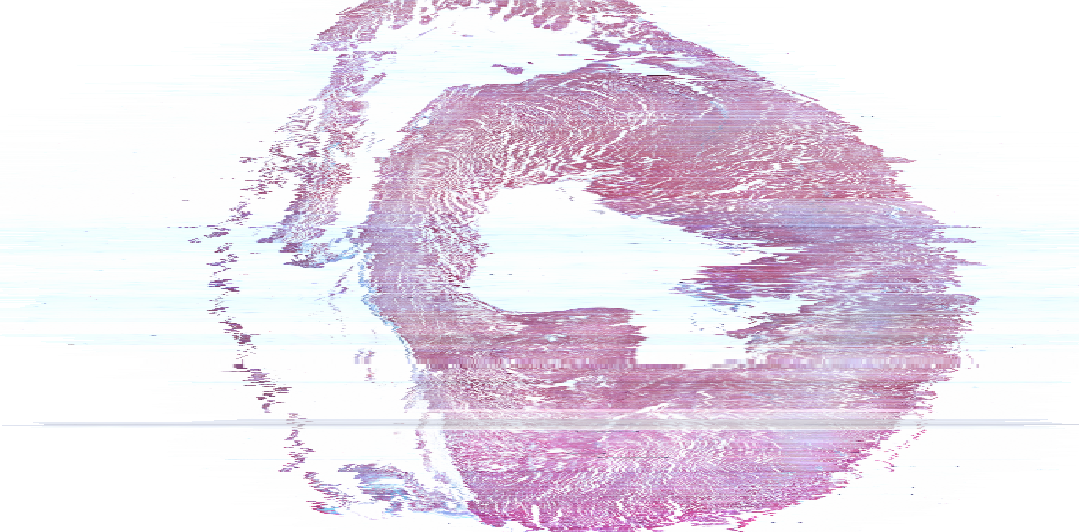
\includegraphics[height=1.2in]{3_results/Figs/banana_1_301}}
    \caption{Cross-sections, located at equivalent locations of (a) the block face volume, (b) the histology slices before registration, aligned to their common geometrical centre, (c) the block face-registered histology slices and (d) the sequentially registered slices with no reference volume.}
    \label{fig:block_face_registration}
  \end{figure}
  Cross-sections of block face, unregistered, block face-registered and serially registered volumes are presented in Figure~\ref{fig:block_face_registration}. We achieve a reasonable large-scale alignment of the great majority of histological slices to form a consistent tissue volume, as is clear from a comparison of Figure~\ref{fig:block_face_registration} (a) and (c). Yet we are left with several limitations of the block face technique. Striations are visible in (a) due to discrete changes in the positioning and intensity of illumination between block face image acquisitions. These changes propagate to the final block face registration result. At the top of the image, large variations in illumination proved excessive for the block-face registration algorithm, and the right ventricle could not be effectively reconstructed. For the left ventricle, the block-face registration seems to produce a successful reconstruction of the volume, when observed at the scale represented in (c). However, when images are observed at full registration, the limitations of the block-face registration are obvious: this is shown in Figure~\ref{fig:vessel_sections}~(a). At 26.6 $\mu$m, the in-plane resolution of the block-face images is 24 times coarser than that of the histology slices (evident in Figure~\ref{fig:raw_images}), precluding an alignment on the scale of cardiac microstructure. This, together with the limitations of the affine transform, the overlap of pixel intensities between tissue and wax, and the interslice variability therein, leads to a noisy, jagged result that is not always at the global minimum.
  
  The sequential slice-to-slice registration in Figure~\ref{fig:block_face_registration}~(d) produces a visually pleasing, smooth reconstruction of the 3D volume. However, as in previous cases it also suffers severely from the banana effect, clearly visible in its deviation from the undistorted reconstruction of block-face images in Figure~\ref{fig:block_face_registration}~(a).
  
  \subsection{TDS on Block Face-Registered Histology} % (fold)
  \label{sub:tds_on_block_face_registered_histology}
  % figure of regional cross-section before smoothing, after global smoothing and after regional smoothing
  \begin{figure}[!t]
    \centering
    \subfloat[]{\includegraphics[width=3.4in]{3_results/Figs/unsmoothed_vessel_1_2125}}\\
    \subfloat[]{\includegraphics[width=3.4in]{3_results/Figs/globally_smoothed_vessel_1_2125}}\\
    \subfloat[]{\includegraphics[width=3.4in]{3_results/Figs/regionally_smoothed_vessel_1_2125}}
    \caption{Central cross sections of the region around an epicardial vessel. Cross-sections are compared before TDS (a), after global application of TDS (b) and after TDS applied locally to this region (c). The blue arrow highlights blue-stained interstitial tissue around vessels, the green arrow epicardial vessels and the yellow arrow enhanced cardiac laminar structure.}
    \label{fig:vessel_sections}
  \end{figure}
  An unmistakable improvement in coherence is observed after global TDS, exemplified in the difference between the images in Figure~\ref{fig:vessel_sections}~(a) and (b). Edges are substantially smoother and the cardiac laminar structure emerges, previously indistinguishable beyond the high-frequency zig-zagging noise. The outer walls are considerably less noisy, and internal vessel walls are much more coherent. However, Figure~\ref{fig:vessel_sections}~(b) is still constrained by the limitations of the affine transform, which in this case is applied globaly. The application of TDS on a regional basis results in the reconstruction shown in Figure~\ref{fig:vessel_sections}~(c), with further improvements in the continuity of paracellular scale structures. 

  % figure of vessel and surface contour before smoothing and after regional smoothing
  \begin{figure*}[!t]
    \centerline{\subfloat[]{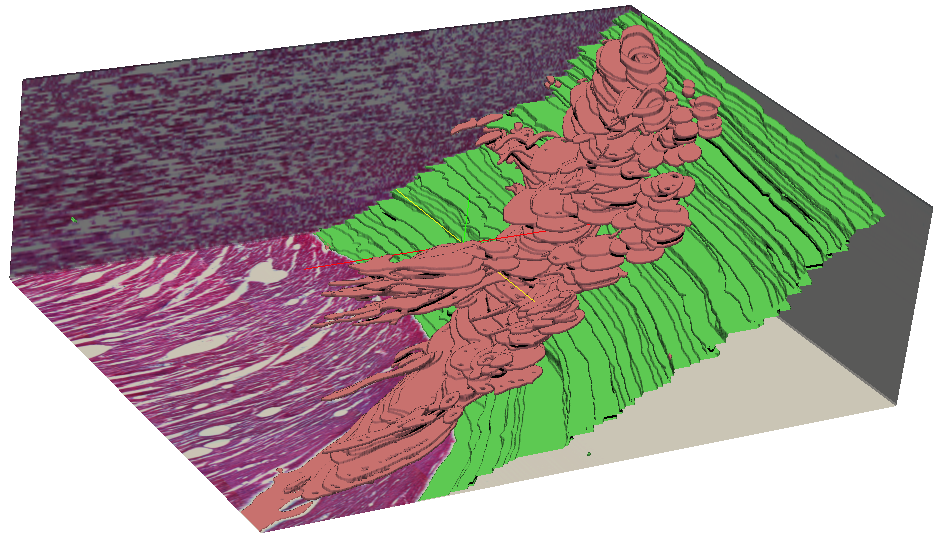
\includegraphics[width=2.4in]{3_results/Figs/unsmoothed_segmentation}} \hfil
    \subfloat[]{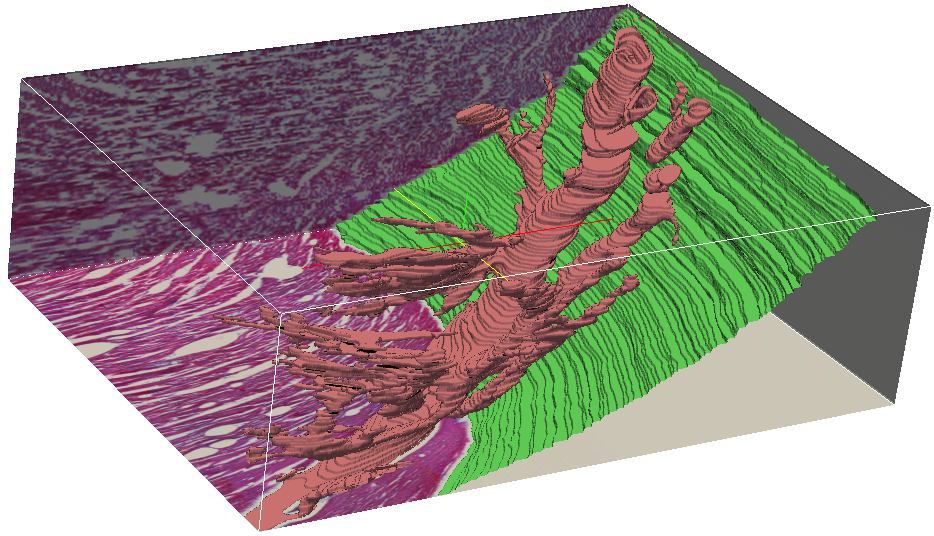
\includegraphics[width=2.4in]{3_results/Figs/globally_smoothed_segmentation}} \hfil
    \subfloat[]{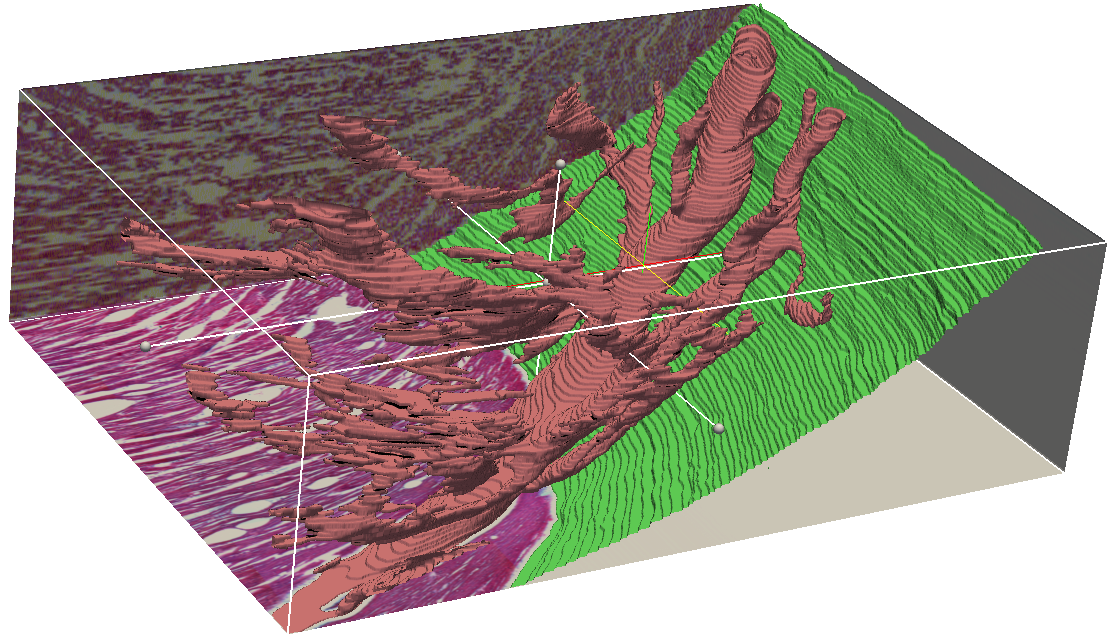
\includegraphics[width=2.4in]{3_results/Figs/locally_smoothed_segmentation}}}
    \caption{Surface contours of segmentations of vasculature (red) and epicardium (green) in the region around an epicardial vessel from Figure~\ref{fig:vessel_sections}, from the unsmoothed, globally smoothed and locally smoothed volumes.}
    \label{fig:region_segmentations}
  \end{figure*} 
  In Figure~\ref{fig:region_segmentations}, progressive enhancement in coherence is visible from the back cross-section, the vessel surface and the pericardial surface, from (a) (unsmoothed) to (b) (after global application of TDS) and then to (c) (after local application of TDS). The contours in (c) are remarkably smooth, with the staircase effects arising only from the inherent thickness of individual slices. In particular, the disturbance near the top of the largest vessel in (b) has been smoothed in (c). Original adjacent slice aberrations in (a) reached $\sim$450$\mu$m. Contrastingly in (c), the relative registration error is reduced below the diameter of even the smallest vessels, by inspection less than 5$\mu$m in the large majority of cases - smaller than the width of a single myocyte. Resultingly, with each of the two smoothing procedures, more of the smaller vasculature has become connected to the main vessel and has been segmented.
    
  % figure of vessel and surface contour before smoothing and after regional smoothing
  \begin{figure}[!t]
    \centering
    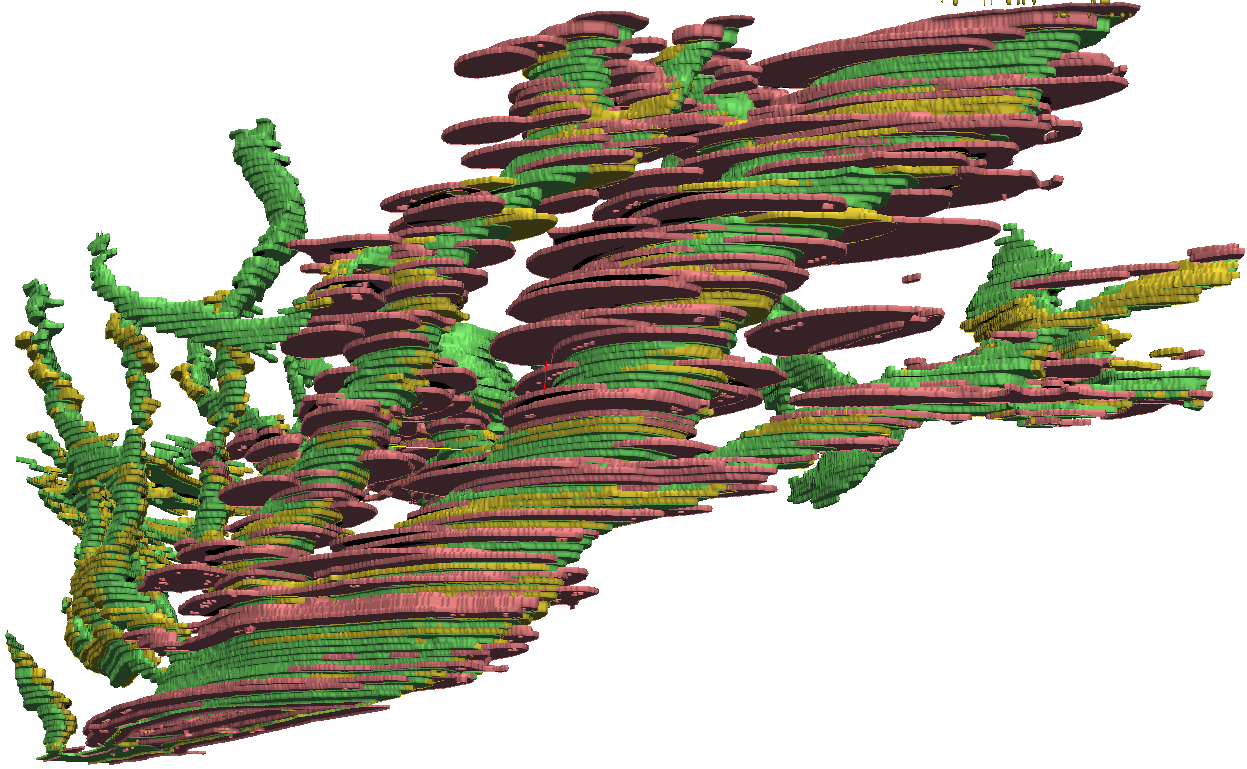
\includegraphics[width=3.4in]{3_results/Figs/vessel_overlay}
    \caption{An overlay of the three vessel segmentations from Figure~\ref{fig:region_segmentations}. The unsmoothed vessel is shaded in red, the globally smoothed vessel in amber and the regionally smoothed vessel in green.}
    \label{fig:vessel_segmentations}
  \end{figure} 
      We see the combined results of all three vascular segmentations (unsmoothed and after global/local TDS) in Figure~\ref{fig:vessel_segmentations}. From this view through the pericardium, the continuity of the green surface is most apparent. The overall shape of the green vessel precisely intersects the disconnected set of red discs, demonstrating that the underlying vessel geometry has been recovered with remarkable accuracy. Again it is clear that the reduction in error below the diameter of the smallest vessels has facilitated their segmentation, with several thin green dendritic structures reaching up into the top left of the figure.  
  % subsection regional_diffusion (end)
% section results (end)
